\documentclass[professionalfont]{beamer}
\usepackage{iftex,ifxetex}
\ifPDFTeX
  \usepackage[utf8]{inputenc}
  \usepackage[T1]{fontenc}
  \usepackage{lmodern}
\else
  \ifluatex
    \usepackage{unicode-math} 
    \defaultfontfeatures{Ligatures=TeX}
    \setmathfont{Latin Modern Math}
    \setsansfont{CMU Sans Serif}
    % \setsansfont{Linux Biolinum O}
  \fi
\fi

\mode<presentation>
{
  \usetheme{Madrid}
  % or ...
  \setbeamertemplate{bibliography item}{}
  \setbeamercovered{transparent}
  % or whatever (possibly just delete it)
}

% \usepackage{fontspec}
\usepackage[english]{babel}
% or whatever
\usepackage{csquotes}
\usepackage[backend=biber,
        style=unified,
        maxcitenames=3,
        maxbibnames=99,
        natbib,
        url=false]{biblatex}
\addbibresource{Dissertation.bib}
% \setmainfont{Linux Libertine O}
% \setmonofont{CMU Typewriter Text}
\renewcommand{\ttdefault}{cmtt}

% \usepackage[colorlinks,allcolors={black},urlcolor={blue}]{hyperref} %allows for hyperlinks and pdf bookmarks 
\usepackage{pifont} %Maths
\usepackage{graphicx}	%Inserting graphics, pictures, images 		
\usepackage{multicol} %Multicolumn text
\usepackage{multirow} %Useful for combining cells in tablesbrew 
\usepackage{booktabs} %Enhanced tables
% \usepackage{underscore} %Allows for underscores in text mode
% \usepackage[colorlinks,allcolors={black},urlcolor={blue}]{hyperref} %allows for hyperlinks and pdf bookmarks
\usepackage{url} %allows for urls
\def\UrlBreaks{\do\/\do-} %allows for urls to be broken up
% \usepackage[normalem]{ulem} %strike out text. Handy for syntax
% \usepackage{tcolorbox}
% \usepackage{datetime2}
% \usepackage{caption}
% \usepackage{subcaption}
\usepackage{tipa} %IPA symbols
% \usepackage{tipauni}
\usepackage{langsci-gb4e} % Language Science Press' modification of gb4e
\usepackage{tikz} % Drawing Hasse diagrams
\usetikzlibrary{decorations.pathreplacing}
\usepackage{leipzig} %	Offers support for Leipzig Glossing Rules

%%MACROS
\newcommand{\sub}[1]{\textsubscript{#1}}
\newcommand{\supr}[1]{\textsuperscript{#1}}
\providecommand{\lsptoprule}{\midrule\toprule}
\providecommand{\lspbottomrule}{\bottomrule\midrule}
\newcommand{\fittable}[1]{\resizebox{\textwidth}{!}{#1}}
\newcommand{\cmark}{\ding{51}}%


\title[Voice Quality in SLZ] % (optional, use only with long paper titles)
{Voice Quality and Laryngeal Complexity in Santiago Laxopa Zapotec}

% \subtitle{Include Only If Paper Has a Subtitle}

\author[Brinkerhoff] % (optional, use only with lots of authors)
{Mykel Loren Brinkerhoff}
% - Give the names in the same order as the appear in the paper.
% - Use the \inst{?} command only if the authors have different
%   affiliation.

\institute[UC Santa Cruz] % (optional, but mostly needed)
{University of California, Santa Cruz}
% - Use the \inst command only if there are several affiliations.
% - Keep it simple, no one is interested in your street address.

\date[2025-06-06] % (optional, should be abbreviation of conference name)
{6 June 2025}
% - Either use conference name or its abbreviation.
% - Not really informative to the audience, more for people (including
%   yourself) who are reading the slides online

% \subject{Theoretical Computer Science}
% This is only inserted into the PDF information catalog. Can be left
% out. 



% If you have a file called "university-logo-filename.xxx", where xxx
% is a graphic format that can be processed by latex or pdflatex,
% resp., then you can add a logo as follows:

\pgfdeclareimage[height=0.5cm]{university-logo}{images/UCSC_Logo_RGB.png}
\logo{\pgfuseimage{university-logo}}



% Delete this, if you do not want the table of contents to pop up at
% the beginning of each subsection:
% \AtBeginSubsection[]
% {
%   \begin{frame}<beamer>{Outline}
%     \tableofcontents[currentsection,currentsubsection]
%   \end{frame}
% }


% If you wish to uncover everything in a step-wise fashion, uncomment
% the following command: 

%\beamerdefaultoverlayspecification{<+->}


\begin{document}

\begin{frame}
  \titlepage
\end{frame}

\begin{frame}{Outline}
  \tableofcontents
  % You might wish to add the option [pausesections]
\end{frame}


% Structuring a talk is a difficult task and the following structure
% may not be suitable. Here are some rules that apply for this
% solution: 

% - Exactly two or three sections (other than the summary).
% - At *most* three subsections per section.
% - Talk about 30s to 2min per frame. So there should be between about
%   15 and 30 frames, all told.

% - A conference audience is likely to know very little of what you
%   are going to talk about. So *simplify*!
% - In a 20min talk, getting the main ideas across is hard
%   enough. Leave out details, even if it means being less precise than
%   you think necessary.
% - If you omit details that are vital to the proof/implementation,
%   just say so once. Everybody will be happy with that.
%-----------------------------------------------------------
\section{Introduction}
%-----------------------------------------------------------
%-----------------------------------------------------------
\subsection{Overview of my dissertation}
%-----------------------------------------------------------

\begin{frame}{Research Overview}
  \begin{block}{Overview:}
    This presentation explores what characterizes voice quality in a Santiago Laxopa Zapotec (SLZ), how is it is structured acoustically, and how this structure helps explain SLZ's laryngeal complexity.  
  \end{block}
\end{frame}

\begin{frame}{Research Overview}
  \begin{block}{Research Questions:}
    \begin{itemize}
      \item How is phonation's acoustic space structured in a single language?
      \item Which measures are important for capturing phonation contrasts?
      \item How do these measures help explain SLZ's laryngeal complexity?
    \end{itemize}
  \end{block}
\end{frame}

\begin{frame}{Research Overview}
  \begin{block}{Answers to Research Questions:}
    \begin{itemize}
      \item The acoustic space is three-dimensional and the dimensions are comparable to \posscitet{keatingCrosslanguageAcousticSpace2023} findings.
      \begin{itemize}
        \item Dimensions are correlated with glottal-airflow (D1/D3) and nonmodal-to-modal (D2) continua.
      \end{itemize}
      \item Only a handful of measures are important for capturing phonation contrasts.
      \item Measures show that SLZ's laryngeal complexity is weakly articulated and shows phasing. 
    \end{itemize}  
  \end{block}
\end{frame}

%-----------------------------------------------------------
\subsection{What is Voice Quality?}
%-----------------------------------------------------------

\begin{frame}{What is Voice Quality?}
  \begin{itemize}
  \item Broad sense $=$ long-term characteristics of an individual's voice \citep{abercrombieElementsGeneralPhonetics1967,laverPhoneticDescriptionVoice1980}.
  \item Narrow sense $=$ how larynx affects phonetic characteristics of speech sounds \citep[e.g.,][]{eslingVoiceQualityLaryngeal2019}.
  \item Sometimes used interchangeably with phonation
    \begin{itemize}
      \item \cite{barzilaiContextdependentPhoneticEnhancement2021} use \textit{voice quality} for phonetic description and \textit{phonation} for phonological contrasts.
    \end{itemize}
  \end{itemize}
\end{frame}

\begin{frame}{How is voice quality used?}
  \begin{itemize}
    \item Paralinguistic information by ``indexing the biological, psychological, and social characteristics of the speaker'' \citep[e.g.,][]{laverVoiceQualityIndexical1968,podesvaStanceWindowLanguageRace2016}
    \item Phonological contrasts \citep[e.g.,][]{espositoCrosslinguisticPatternsPhonation2020}.
  \end{itemize}
\end{frame}

\begin{frame}{Why study voice quality?}
  \begin{itemize}
    \item Voice quality plays a crucial role in speech communication.
    \item It is used in many languages to create phonological contrasts.
    \item It is a rich area of research that can help us understand speech production and perception.
  \end{itemize}
\end{frame}

%-----------------------------------------------------------
\subsection{Santiago Laxopa Zapotec}
%-----------------------------------------------------------

\begin{frame}{What is Santiago Laxopa Zapotec}
  \begin{columns}
    \begin{column}{0.33\textwidth}
      \begin{itemize}
        \item Santiago Laxopa Zapotec (SLZ; \textit{Dille'xhunh Laxup}) is a Sierra Norte variety of Zapotec (Oto-Manguean).
        \item Spoken by c. 1,000 speakers in Santiago Laxopa and in diaspora.
      \end{itemize}
    \end{column}
    \begin{column}{0.67\textwidth}
      \begin{figure}
        \centering
        \includegraphics[width=0.95\linewidth]{images/Oaxaca_Santiago_Laxopa_Map.eps}
      \end{figure}
    \end{column}
  \end{columns}
\end{frame}

\begin{frame}{Why study SLZ?}
  \begin{itemize}
        \item SLZ is a relatively understudied language, so it provides an opportunity to contribute to our linguistic understaning.
    \item SLZ has a complex laryngeal system that is not well understood.
    \begin{itemize}
      \item SLZ has a four-way phonation contrast.
      \item SLZ has a five-way tonal contrast.
      \item These contrasts are orthogonal, meaning that they can occur independently of each other.
    \end{itemize} 
  \end{itemize}
\end{frame}

\begin{frame}{Phonation in SLZ}
  \begin{itemize}
    \item SLZ has a four-way phonation contrast:
    \begin{itemize}
      \item Modal ( [\textipa{a}] )
      \item Breathy ( [\textipa{\"*a}] )
      \item Checked ( [\textipa{\t{aP}}] or [\textipa{\t{a\~*a}}] )
      \item Rearticulated ([\textipa{\t{aPa}}], [\textipa{\t{a\~*aa}}], or [\textipa{\~*a}] )
    \end{itemize}
  \end{itemize}
\end{frame}

\begin{frame}{Breathy Phonation in SLZ}
  \begin{columns}
    \begin{column}{0.33\linewidth}
      \begin{itemize}
        \item Characterized by aperiodicity and noise in the harmonic structure.
        \item Longer duration than modal voice
        \item Lower fundamental frequency (\textit{f}0)
      \end{itemize}  
    \end{column}

    \begin{column}{0.67\linewidth}
      \begin{figure}[h!]
        \centering
        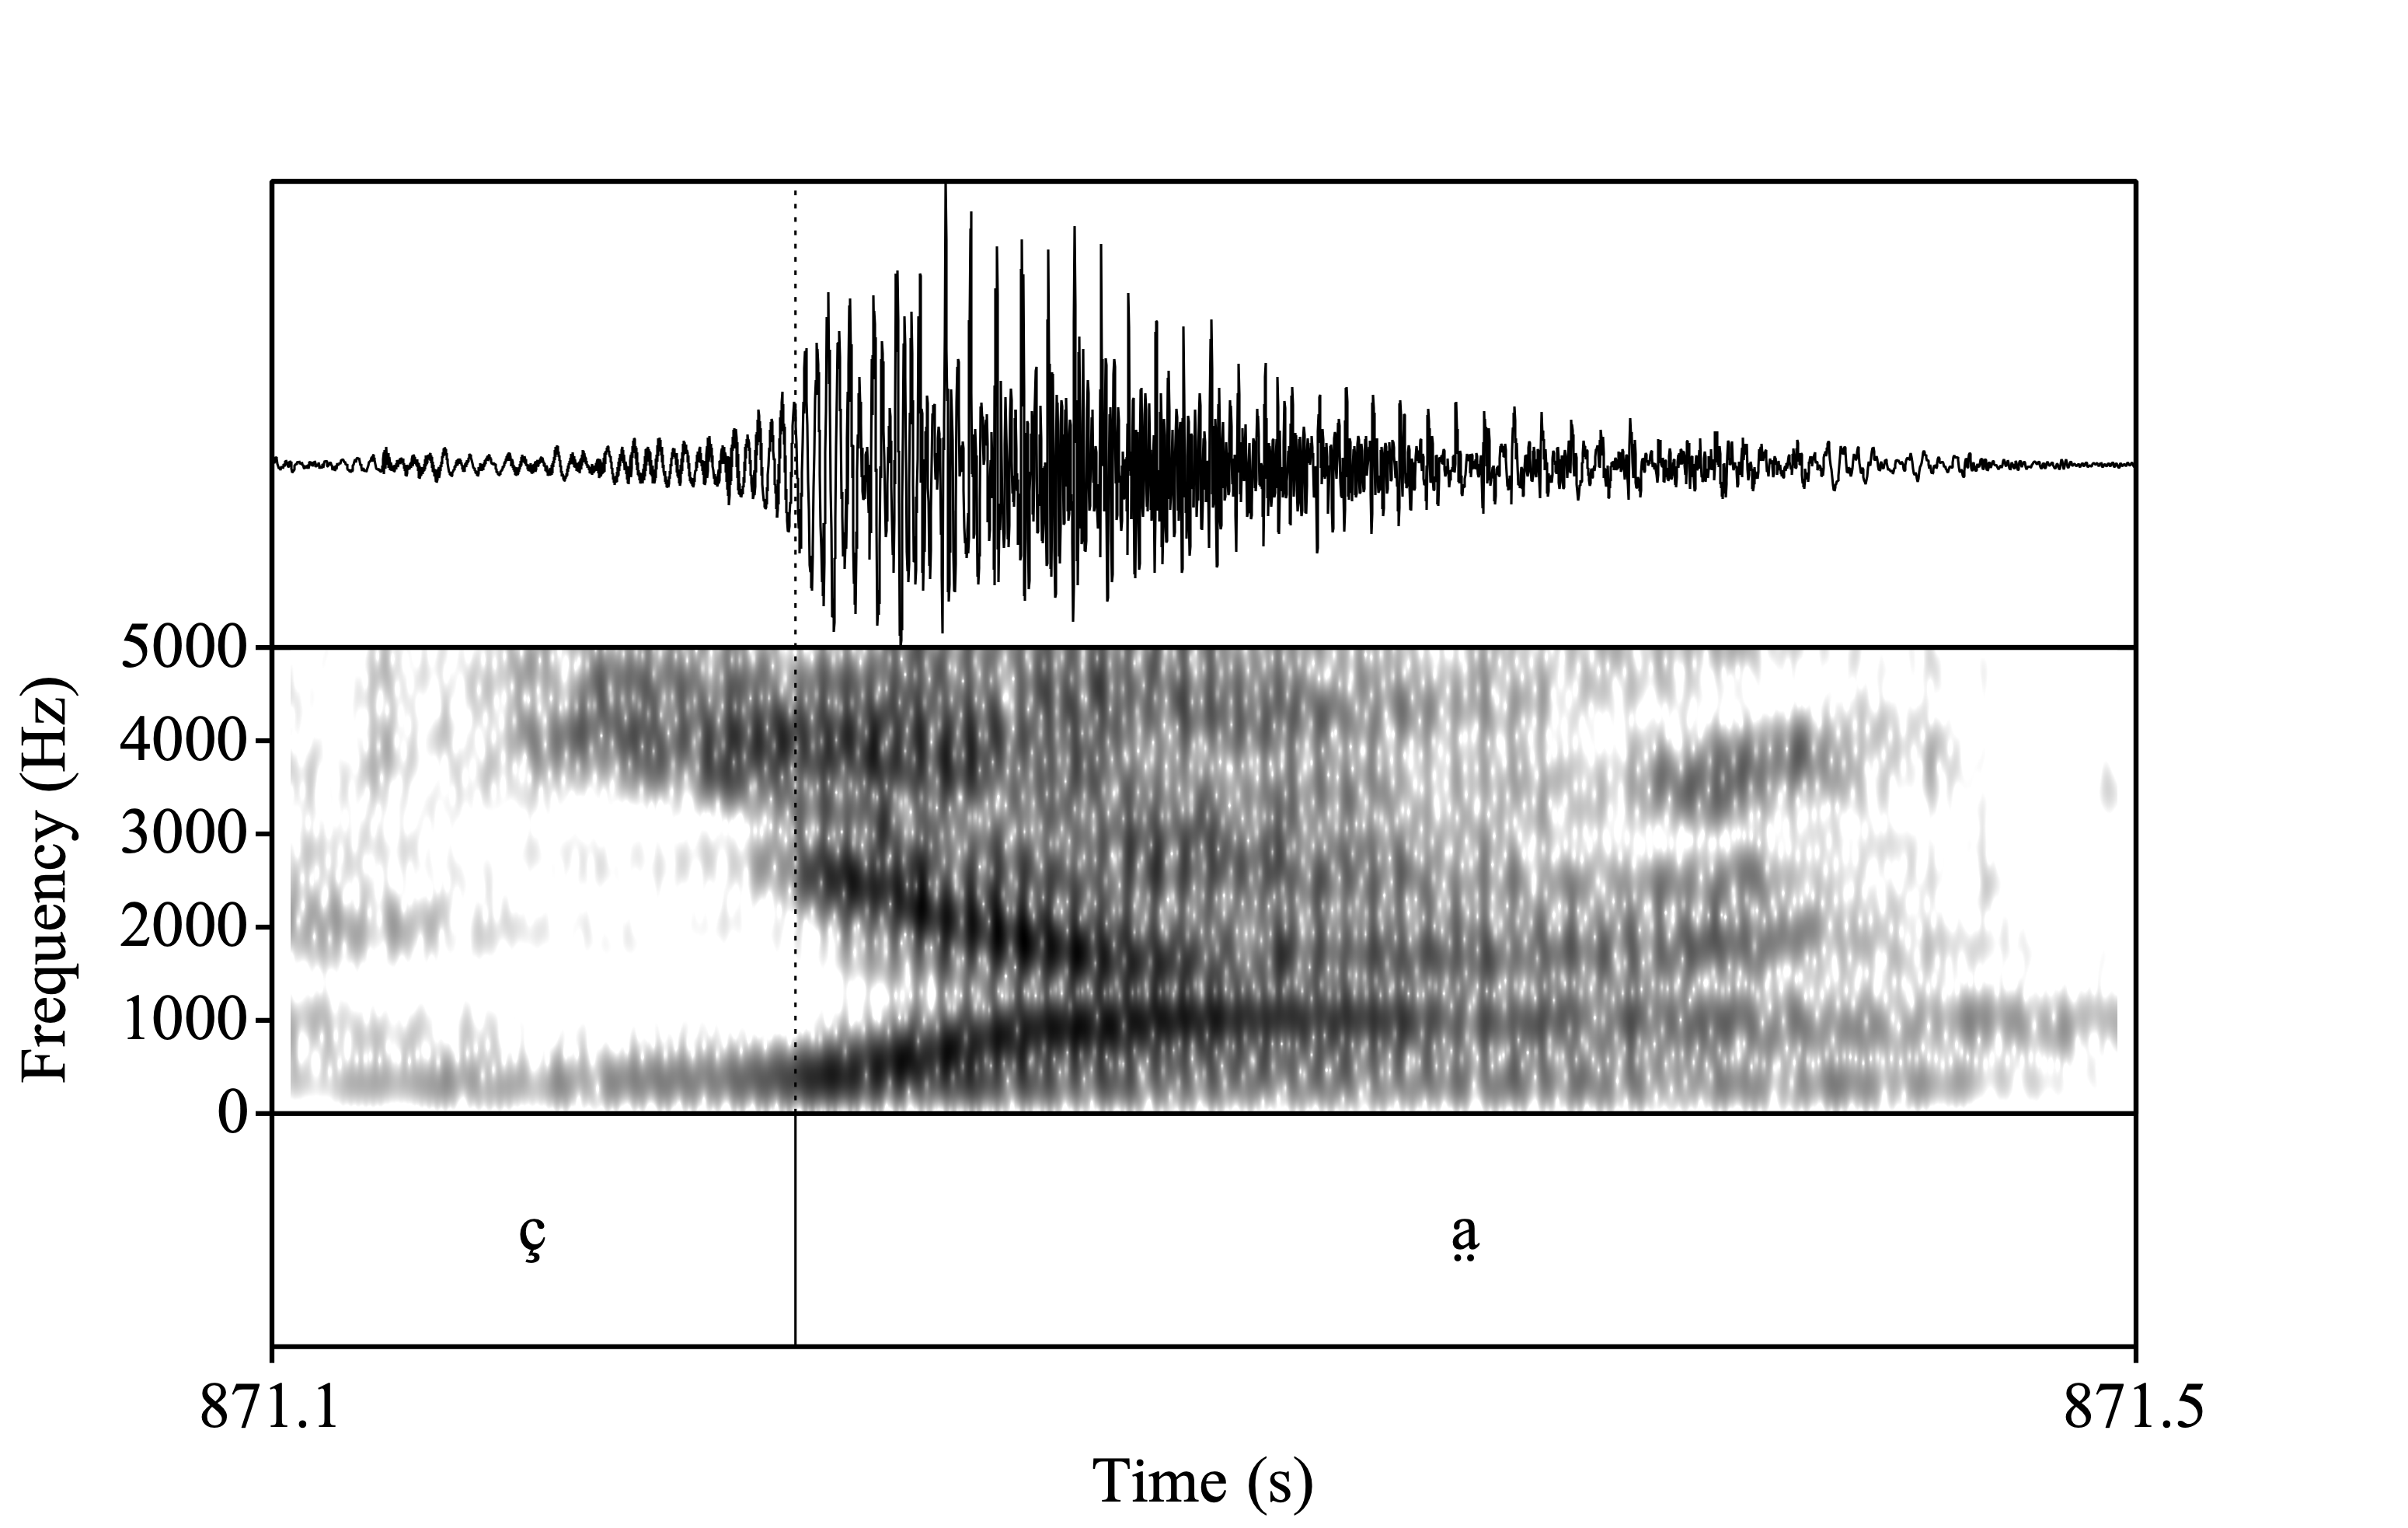
\includegraphics[width=\textwidth]{images/Spectrograms/yah.png}
      \end{figure}
    \end{column}
  \end{columns}
\end{frame}

\begin{frame}{Checked Phonation in SLZ}
  \begin{columns}
    \begin{column}{0.33\linewidth}
      \begin{itemize}
        \item Glottal occlusion at the end of vowel or creaky voice in second half vowel.
        \item Decrease in voicing amplitude during second half.
      \end{itemize}  
    \end{column}

    \begin{column}{0.67\linewidth}
      \begin{figure}[h!]
        \centering
        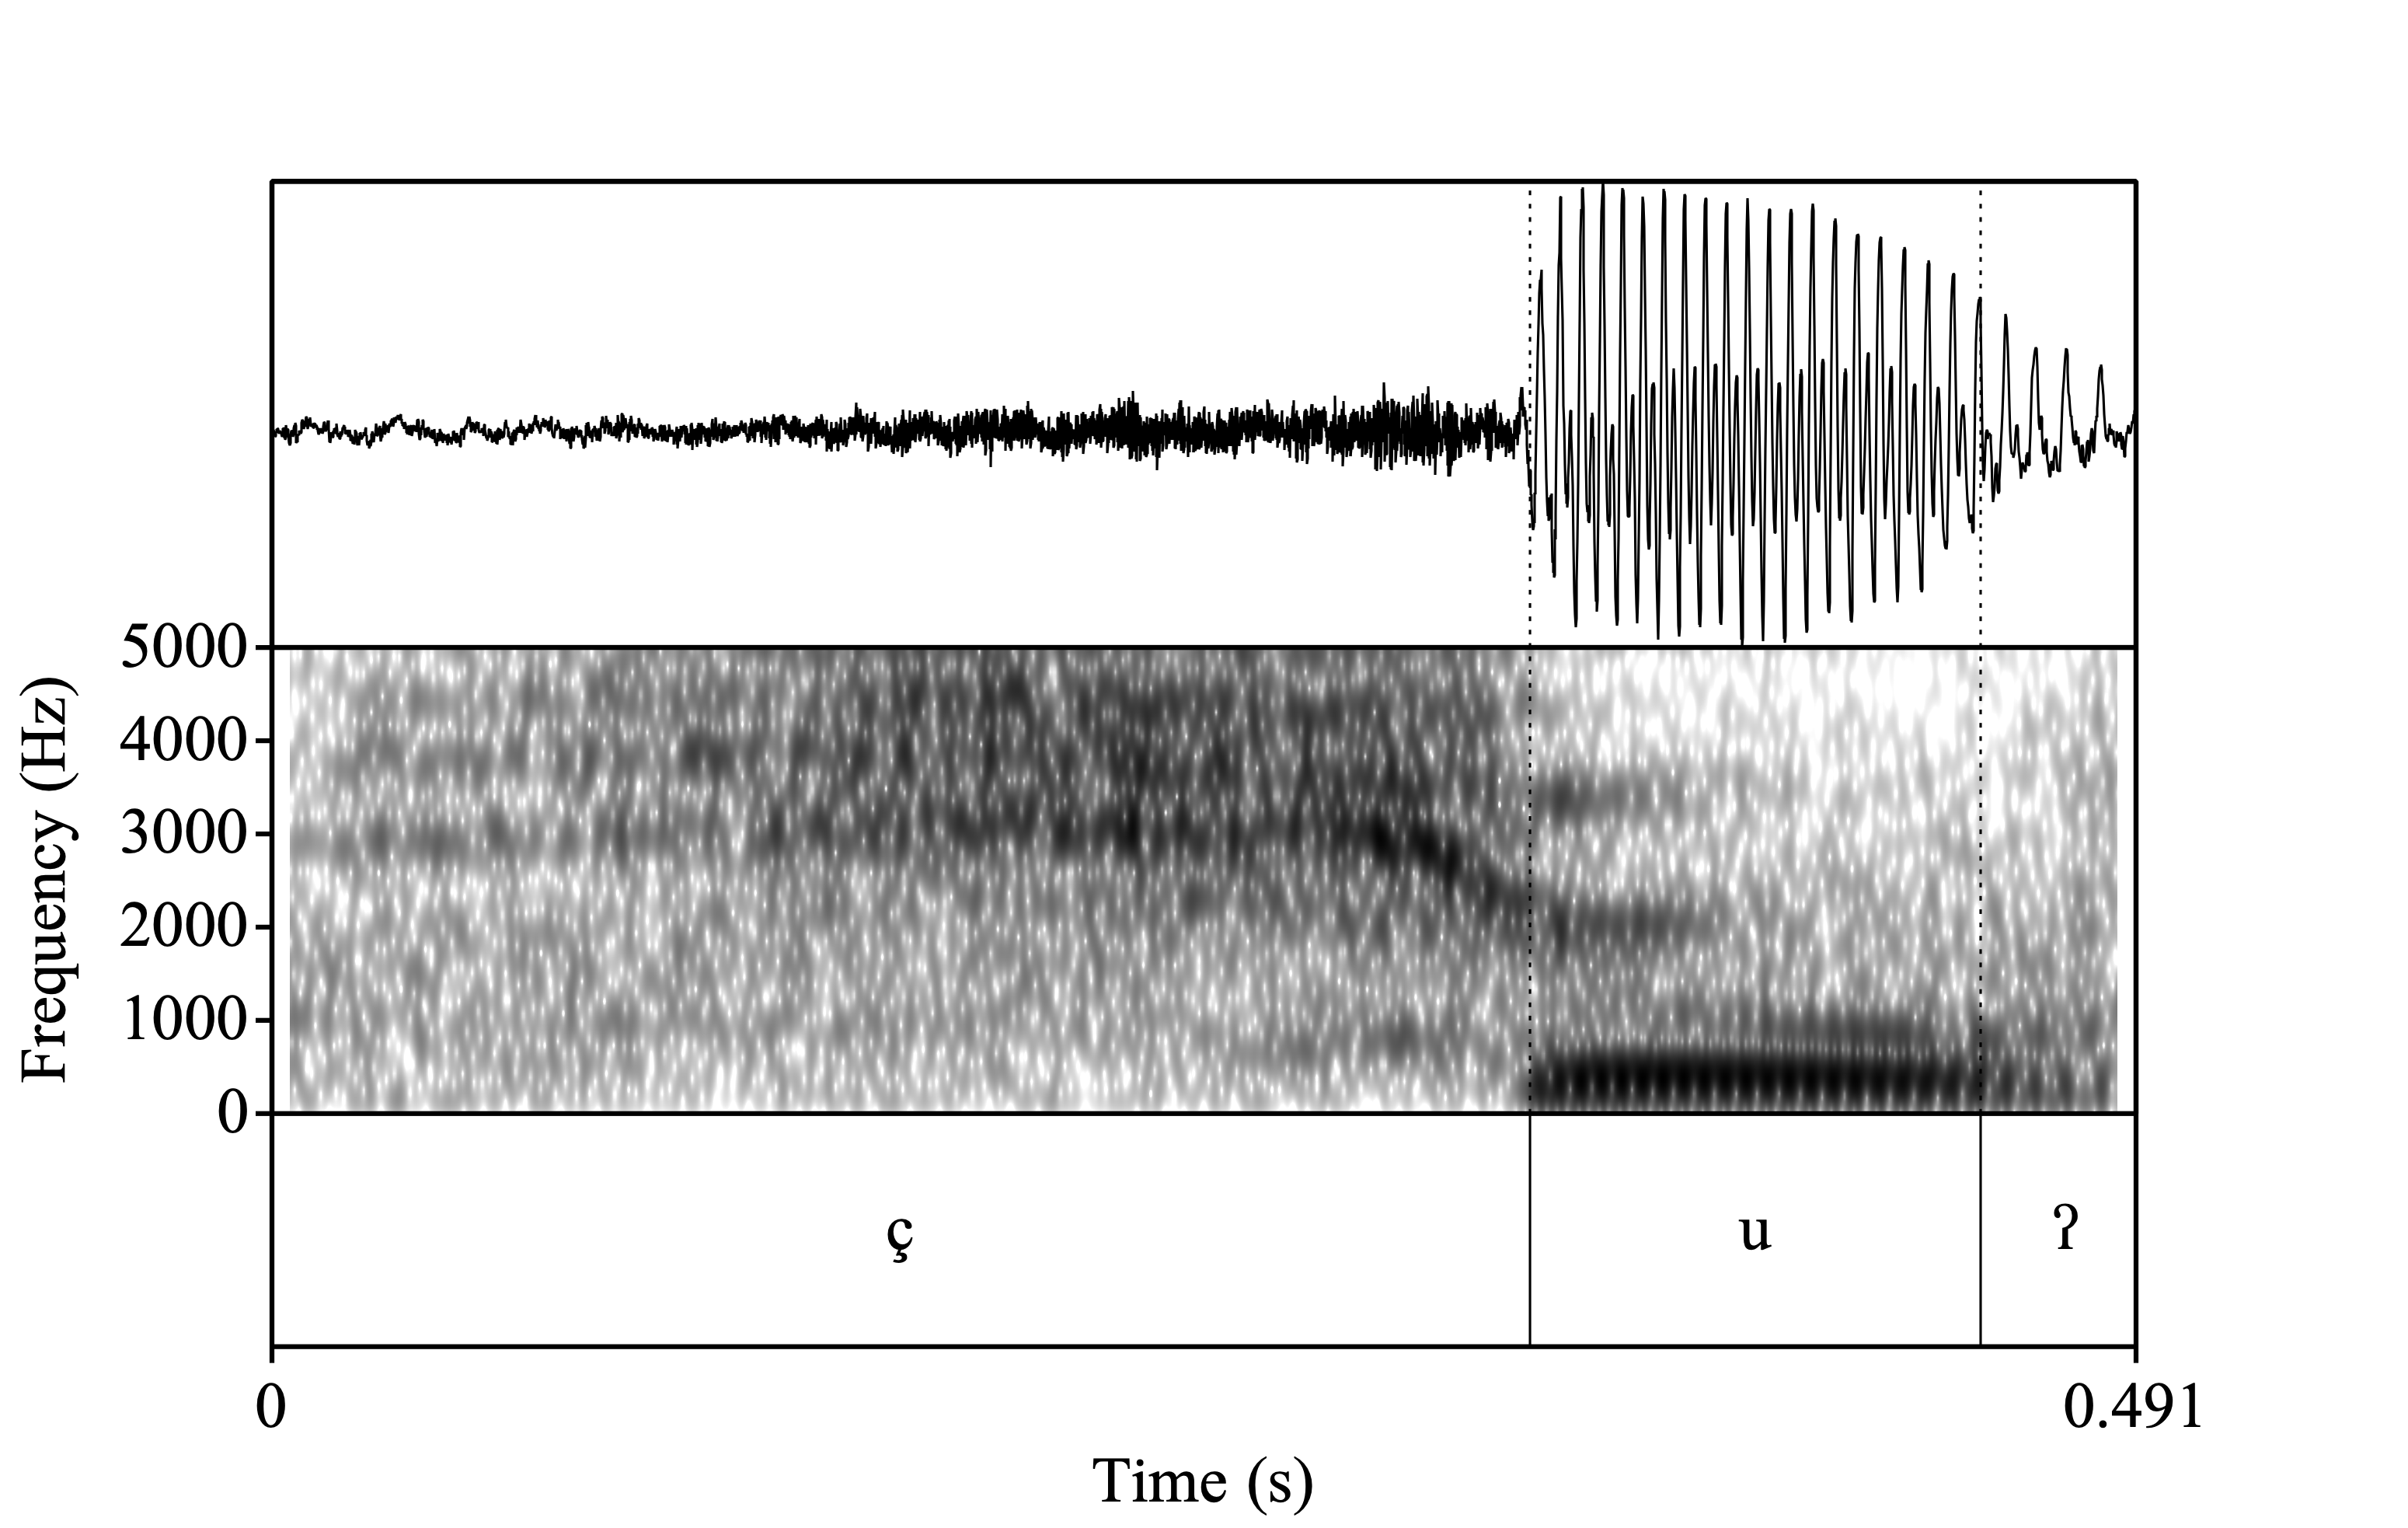
\includegraphics[width=\textwidth]{images/Spectrograms/RD_yu'.png}
      \end{figure}
    \end{column}
  \end{columns}
\end{frame}

\begin{frame}{Rearticulated Phonation in SLZ}
  \begin{columns}
    \begin{column}{0.33\linewidth}
      \begin{itemize}
        \item Glottal occlusion or creaky voice in the middle of the vowel.
        \item Longer duration than modal voice
        \item Decrease in voicing amplitude during first half.
      \end{itemize}  
    \end{column}

    \begin{column}{0.67\linewidth}
      \begin{figure}[h!]
        \centering
        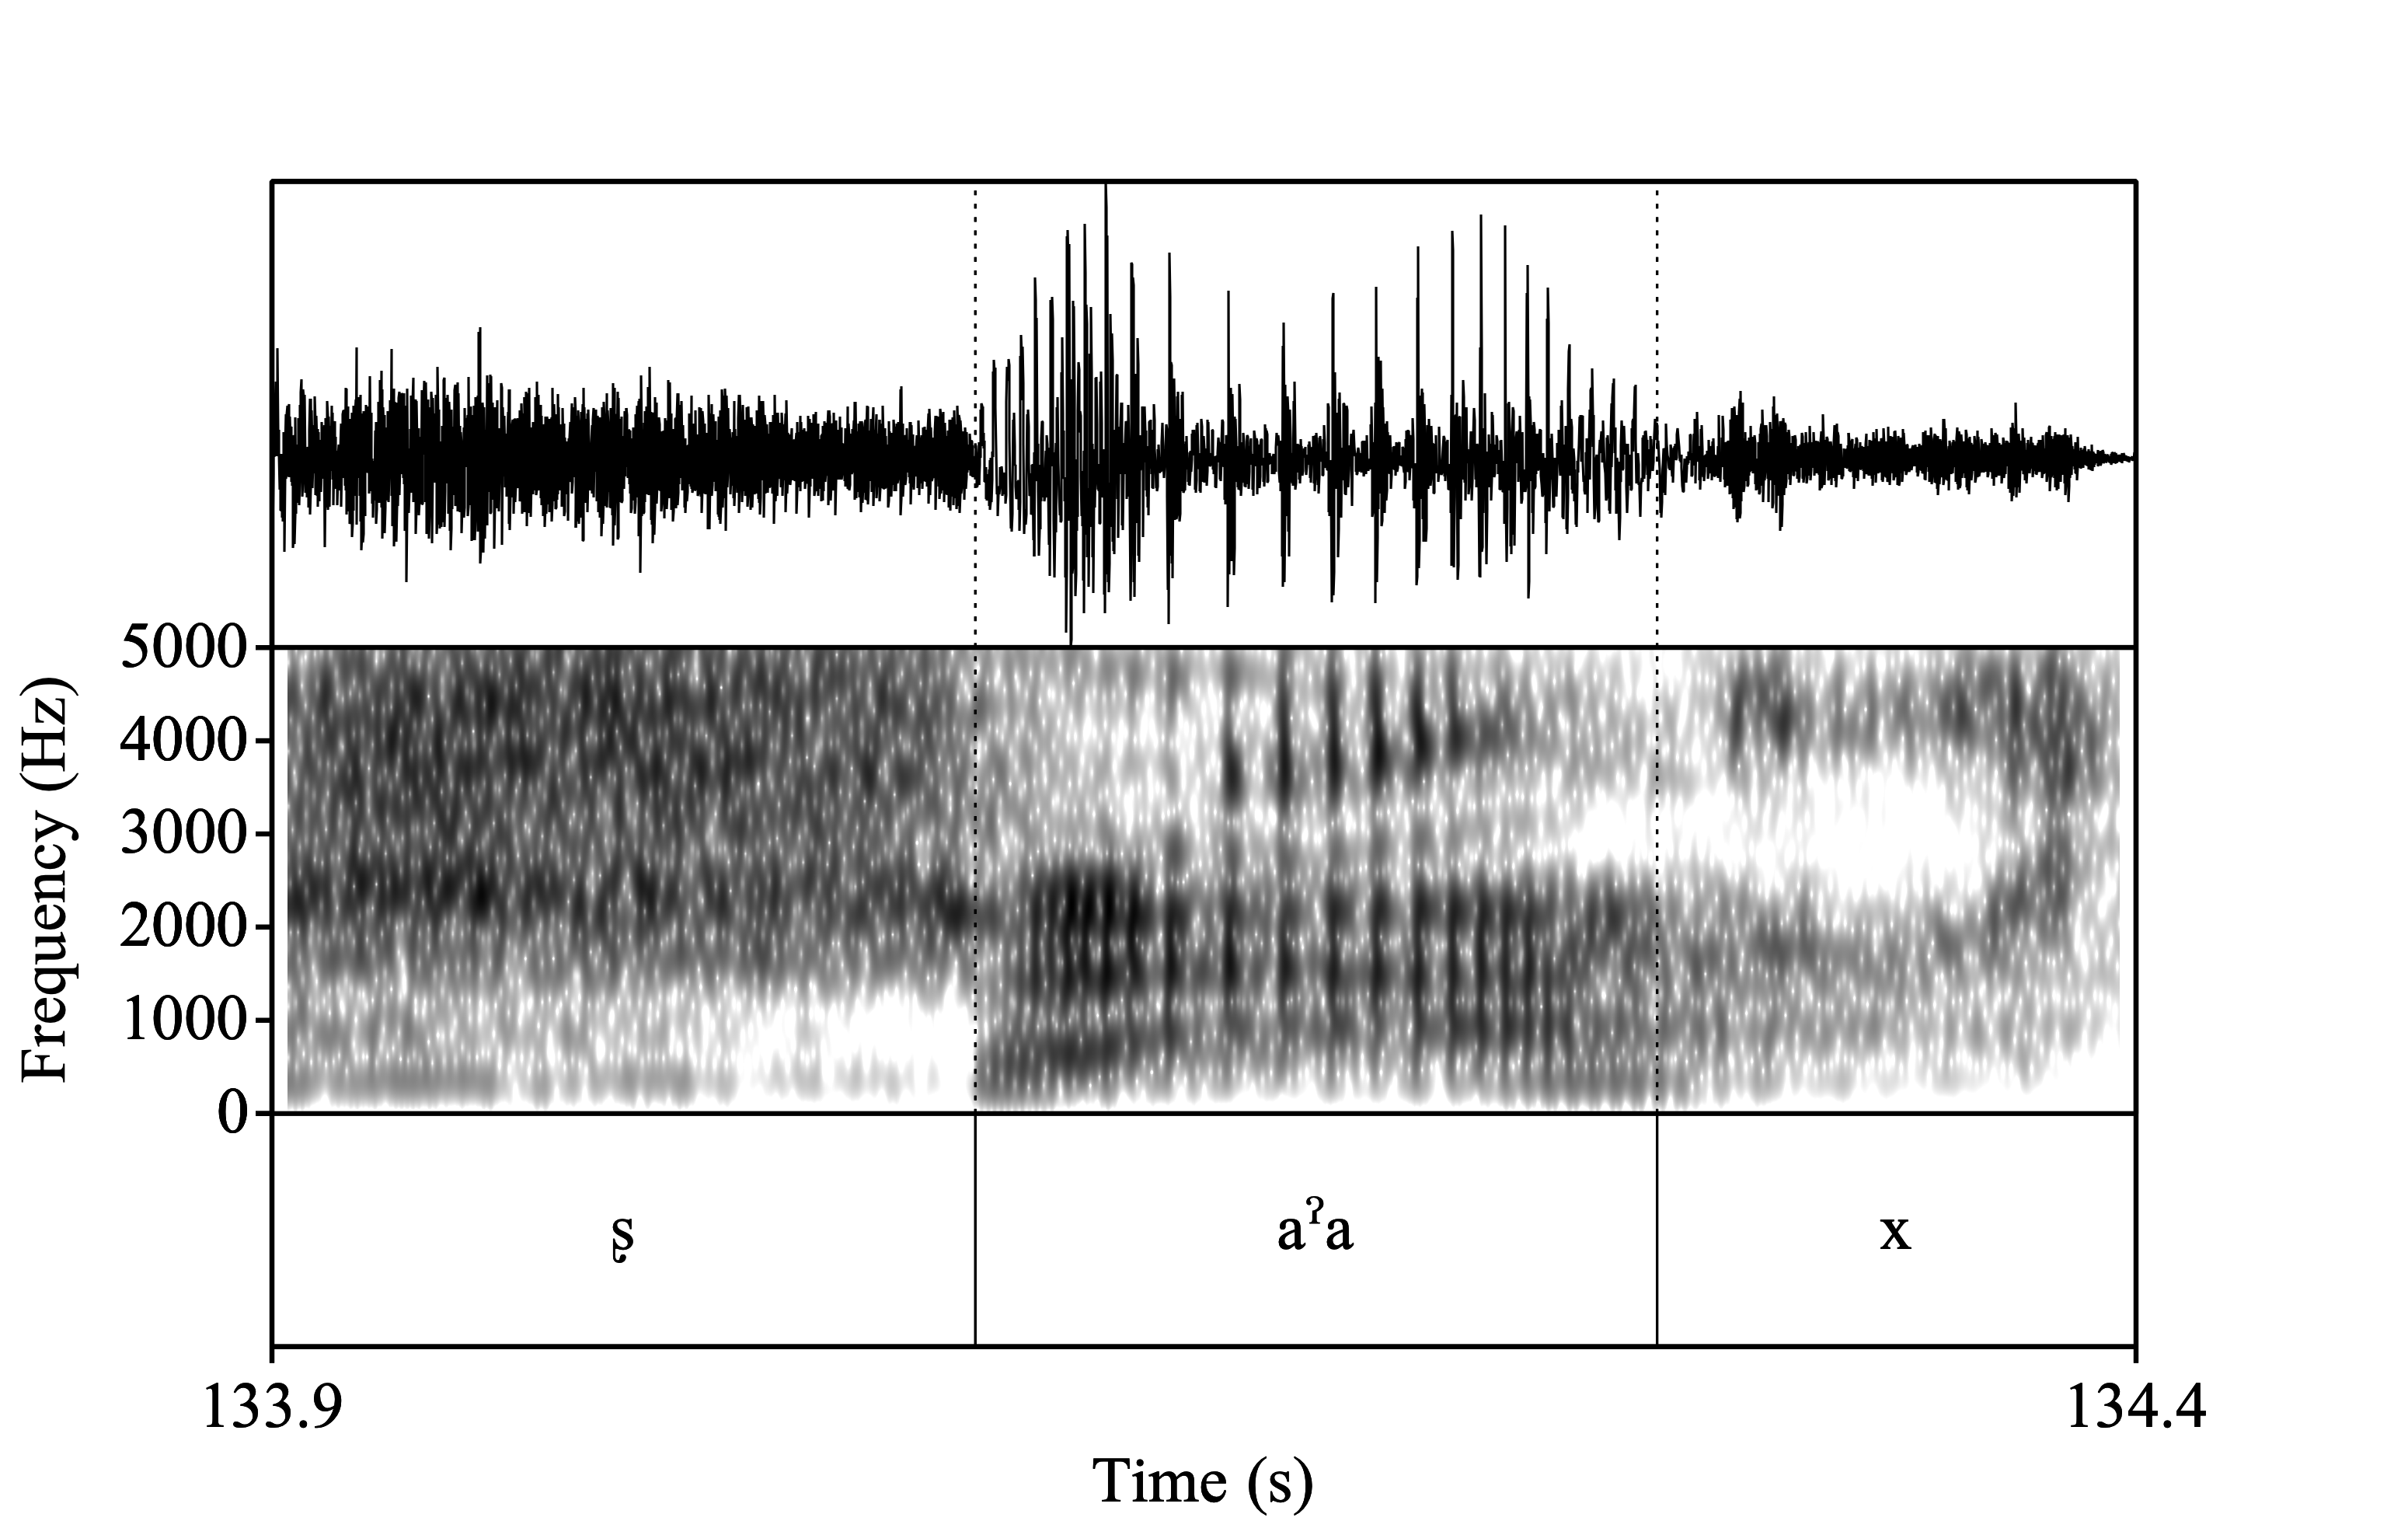
\includegraphics[width=\textwidth]{images/Spectrograms/xa'ag.png}
      \end{figure}
    \end{column}
  \end{columns}
\end{frame}

\begin{frame}{Tone in SLZ}
  \begin{itemize}
    \item SLZ shows a five-way tonal contrast on monosyllabic nouns \citep{brinkerhoffTonalPatternsTheir2022}.
  \end{itemize}
  \begin{table}[!h]
	  \centering
	  \begin{tabular}{llll}
	    \lsptoprule
					  % &	 Diacritic  & Example & Transcription \\
	    High   	 &  \textit{xha}   &  [ ʐa˦ ] & `clothing.\Poss{}'\\
	    Mid    	 &  \textit{lhill} 	& [ ɾiʒ˧ ] & `house.\Poss{}' \\
	    Low   	 &  \textit{yu'} 	& [ çuˀ˨ ] & `earth'\\
	    Rising	 &  \textit{yu'u} 	& [ çuˀu˧˦ ] & `lime (Sp. \textit{cal})' \\
	    Falling  &  \textit{yu'u}  &  [ çuˀu˦˨ ] &	`house' \\
	    \lspbottomrule
	  \end{tabular}
\end{table}
\end{frame}

\begin{frame}{Interaction of Tone and Phonation in SLZ}
  \begin{itemize}
    \item Tone and phonation are orthogonal in SLZ.
  \end{itemize}
  \begin{table}[h!]
	\centering
	  \begin{tabular}{lcccc}
	    \lsptoprule
		  & \textbf{Modal} & \textbf{Breathy} & \textbf{Checked} & \textbf{Rearticulated} \\
	    \hline
	    High		& \cmark & -- & \cmark & \cmark \\
	    Mid			& \cmark & \cmark & \cmark & \cmark \\
	    Low			& \cmark & \cmark & \cmark & \cmark \\
	    Rising	& \cmark & \cmark & -- & \cmark \\
      Falling	& \cmark & \cmark & \cmark & \cmark \\
	    \lspbottomrule
	  \end{tabular}
  \end{table} 
\end{frame}

%-----------------------------------------------------------
\section{Previous research}
%-----------------------------------------------------------
% \frame{\sectionpage}
%-----------------------------------------------------------
\subsection{Measuring Voice Quality}
%-----------------------------------------------------------

\begin{frame}{Measuring voice quality}
  \begin{itemize}
    \item Long been established that phonation has correlates in the acoustic signal (e.g., \cite{fischer-jorgensenPhoneticAnalysisBreathy1968,klattAnalysisSynthesisPerception1990}).
    \item \citet{fischer-jorgensenPhoneticAnalysisBreathy1968} found that a strengthened fundamental (i.e., H1) correlated with breathy vowels in Gujarati.
    \begin{itemize}
      \item Proposed H1$-$H2 amplitude as a measure to normalize for overall intensity differences
    \end{itemize}
    \item Subsequent research has shown that H1$-$H2 is useful for classifying voice quality contrasts.  
    \item However, it is not without its problems (see \cite{chaiH1H2AcousticMeasure2022} for an overview).
  \end{itemize}
\end{frame}

\begin{frame}{Measuring voice quality}
  \begin{itemize}
    \item H2 and other normalizations (A1, A3) are really attempts to understand the relative strength of the fundamental (H1) to higher harmonic energy
    \item H1 and H2 are affected by subglottal pressure differently \citep{sundbergObjectiveCharacterizationPhonation2022}
    \begin{itemize}
      \item This undermines the original reasoning behind H1$-$H2
    \end{itemize} 
    \item Researchers sometimes find that H1$-$H2 does not distinguish phonation types \citep[e.g.,][]{espositoVariationContrastivePhonation2010,espositoAcousticElectroglottographicStudy2012,garellekPhoneticsWhiteHmong2023}.
    \item Error in measuring H1$-$H2 is uncomfortably high \citep[e.g.,][]{chaiH1H2AcousticMeasure2022}.
  \end{itemize}
\end{frame}

\begin{frame}{Measuring voice quality}
  \begin{itemize}
    \item Many measures have been proposed to capture voice quality.
    \item Measures can be broadly categorized into several categories \citep{gordonPhonationTypesCrosslinguistic2001}:
    \begin{itemize}
      \item Periodicity (e.g., HNR or CPP)
      \item Energy 
      \item Spectral tilt (e.g., H1*$-$H2*, residual H1*)
      \item Pitch (e.g., \textit{f}0)
      \item Duration 
    \end{itemize}
  \item Linguists have used combinations of these measures to model phonation (e.g., \cite{blankenshipTimingNonmodalPhonation2002,brunelleTonePhonationSoutheast2016,espositoAcousticElectroglottographicStudy2012}).
  \end{itemize}
\end{frame}

\begin{frame}{New measures of voice quality}
  \begin{itemize}
    \item New measures are being developed all the time.
    \item \posscitet{chaiH1H2AcousticMeasure2022} residual H1* is a new measure of spectral tilt that is more robust than traditional spectral tilt measures.
    \begin{itemize}
      \item Does this by removing the the effects of Energy from the H1* measure.
      \item This was the original goal of \citet{fischer-jorgensenPhoneticAnalysisBreathy1968}
    \end{itemize}
    \item \citet{brinkerhoffUsingResidualH12025} found that residual H1* is a better measure of spectral tilt than H1*$-$H2* for Santiago Laxopa Zapotec's four-way phonation contrast.
  \end{itemize}
\end{frame}

\begin{frame}{Too many measures}
  \begin{itemize}
    \item There are many measures of voice quality, but it is not clear which ones are the most useful.
    \item It also makes it difficult to compare results across studies.
    \item VoiceSauce makes this a common issue \citep{shueVoiceSauceProgramVoice2011}.
  \end{itemize}
\end{frame}

\begin{frame}{Too many measures}
  \begin{itemize}
    \item \citet{kreimanUnifiedTheoryVoice2014,kreimanValidatingPsychoacousticModel2021} tackle this by proposing a psychoacoustic model of voice quality.
    \item Found certain measures are perceptually more important than others.
  \end{itemize}
  \begin{table}[h!]
    \centering
    % \caption{Components of the psychoacoustic model of voice quality and associated voice synthesis parameters.}
    \fittable{
    \begin{tabular}{|l|l|}
    \hline
    \textbf{Model Component} & \textbf{Parameters} \\
    \hline
    \multirow{4}{*}{Harmonic source spectral shape} 
      & H1--H2 \\
      & H2--H4 \\
      & H4--2~kHz \\
      & 2~kHz--5~kHz \\
    \hline
    Inharmonic source excitation 
      & Spectrally-shaped noise-to-harmonics ratio \\
    \hline
    \multirow{2}{*}{Time-varying source characteristics} 
      & $f0$ mean and standard deviation (or $f0$ track) \\
      & Amplitude mean and standard deviation (or amplitude track) \\
    \hline
    \multirow{2}{*}{Vocal tract transfer function} 
      & Formant frequencies/bandwidths \\
      & Spectral zeroes/bandwidths \\
    \hline
    \end{tabular}}
  \end{table}
\end{frame}

%-----------------------------------------------------------
\subsection{Modeling Voice Quality}
%-----------------------------------------------------------


\begin{frame}{Modeling voice quality}
  \begin{itemize}
    \item Early models proposed that voice quality is one dimensional and represents glottal airflow \citep{ladefogedPreliminariesLinguisticPhonetics1971,ladefogedSoundsWorldsLanguages1996}.
  \end{itemize}
  \begin{figure}[h!]
    % \centering
    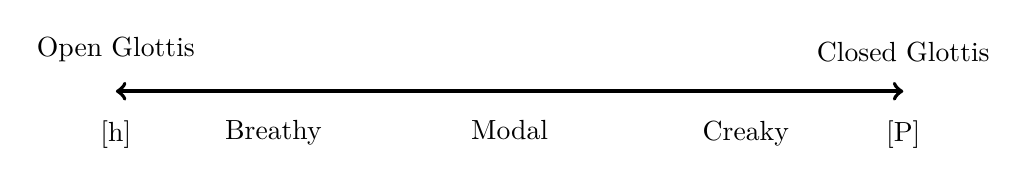
\begin{tikzpicture}
        % Draw the line with arrows at both ends
        \draw[<->, line width=0.5mm] (0,0) -- (10,0);
        
        % Labels underneath the line
        \node[below, yshift=-0.25cm] at (0,0) {[\textipa{h}]};
        \node[below, yshift=-0.25cm] at (2,0) {Breathy};
        \node[below, yshift=-0.25cm] at (5,0) {Modal};
        \node[below, yshift=-0.25cm] at (8,0) {Creaky};
        \node[below, yshift=-0.25cm] at (10,0) {[\textipa{P}]};
        
        % Labels above the line
        \node[above, yshift=0.25cm] at (0,0) {Open Glottis};
        \node[above, yshift=0.25cm] at (10,0) {Closed Glottis};
    \end{tikzpicture}
    % \caption{A diagram showing the relationship between breathy, modal, and creaky phonation types from \citet{gordonPhonationTypesCrosslinguistic2001}.}
    % \label{fig:phonation_types}
\end{figure}
\end{frame}

\begin{frame}{Voice quality's multidimensionality}
  \begin{itemize}
    \item More recent work has shown that voice quality is not one-dimensional, but minimally five-dimensional \citep[e.g.,][]{garellekModelingVoiceSource2016,kreimanValidatingPsychoacousticModel2021}.
    \begin{itemize}
      \item Especially in the case of individual speaker differences.
    \end{itemize}
    \item \citet{garellekVoiceQualityTone2013} has argued that dimensionality might not be as complex for capturing phonation contrasts.
  \end{itemize}
\end{frame}

\begin{frame}{\citet{keatingCrosslanguageAcousticSpace2023}}
  \begin{itemize}
    \item Explored phonation's cross-linguistic acoustic space.
    \item Found a two-dimensional space for phonation across 11 languages.
    \begin{enumerate}
      \item First dimension $=$ nonmodal-to-modal continuum.
      \item Second dimension $=$ glottal-airflow continuum.
    \end{enumerate}
    \item Found languages with more contrasts used more of the acoustic space than languages with fewer contrasts.
    \item Found correlations between dimensions and acoustic measures.
    \begin{enumerate}
      \item First dimension $=$ periodicity and energy measures.
      \item Second dimension $=$ spectral tilt and periodicity measures.
    \end{enumerate}
  \end{itemize}
\end{frame}

\begin{frame}{\citet{keatingCrosslanguageAcousticSpace2023}}
  \begin{figure}[h!]
    \centering
    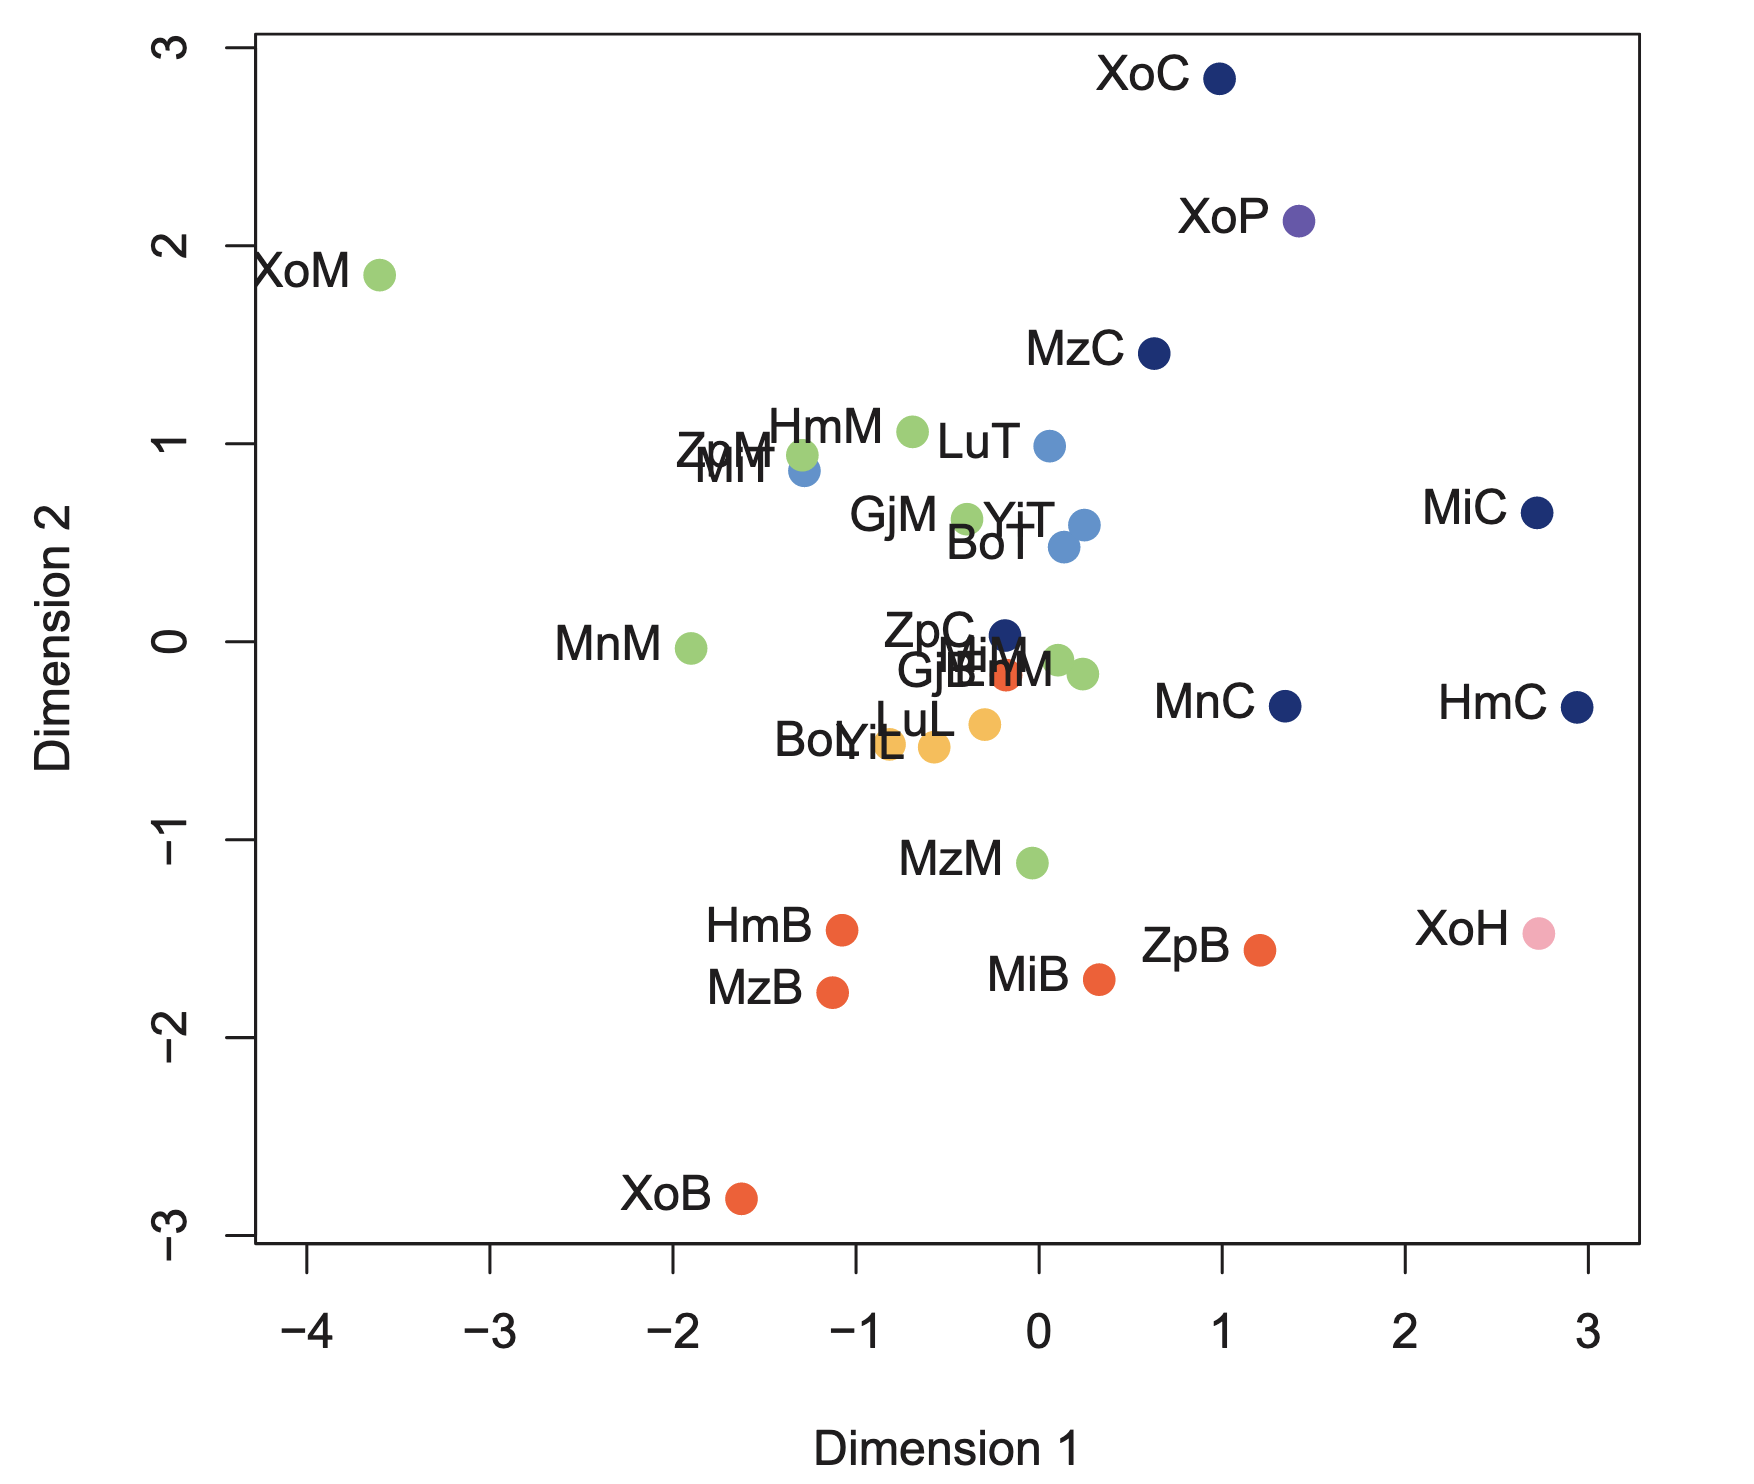
\includegraphics[width = 0.8\linewidth]{images/Keating_dimension.png}
  \end{figure}
\end{frame}

%-----------------------------------------------------------
\subsection{Laryngeal Complexity}
%-----------------------------------------------------------

\begin{frame}{What is Laryngeal Complexity}
  \begin{itemize}
    \item \textit{Laryngeal complexity} describes languages that use both contrastive tone and phonation \citep{silvermanLaryngealComplexityOtomanguean1997,silvermanPhasingRecoverability1997}.
    \item Very common in the Oto-Manguean language family, but is also found in other languages.
  \end{itemize}
\end{frame}

\begin{frame}{Phonation's phasing}
  \begin{itemize}
    \item 
  \end{itemize}
\end{frame}

\begin{frame}{Implicational hierarchy of patterns}
  \begin{itemize}
    \item \citet{silvermanLaryngealComplexityOtomanguean1997} proposed a hierarchy of laryngeal complexity phasing pattern.
  \end{itemize}
  \begin{table}[h!]
%     \centering
%     % \caption{Implicational hierarchy of laryngeal complexity. The symbols h and ʔ represent laryngealization. The symbol V represents where the modal vowel is located in relation to the laryngealization. Modified from \citet{silvermanLaryngealComplexityOtomanguean1997}.} 
    % \label{tab:implicational_hierarchy}
    \begin{tabular}{lccc}
        \lsptoprule
        \textbf{Language} & \textbf{Prevocalic} & \textbf{Postvocalic} & \textbf{Interrupted} \\
        \hline 
        Jalapa Mazatec & hV˥, ʔV˥ & $-$ & $-$ \\
        Comaltepec Chinantec & hV˥, ʔV˥ & Vh˥, Vʔ˥ & $-$ \\
        Copala Trique & hV˥, ʔV˥ & Vh˥, Vʔ˥ & VhV˥, VʔV˥ \\
        \lspbottomrule
    \end{tabular}
\end{table}
\end{frame}

\begin{frame}{Previous research on laryngeal complexity}
  \begin{itemize}
    \item 
  \end{itemize}
\end{frame}

%-----------------------------------------------------------
\section{My Results}
%-----------------------------------------------------------
%-----------------------------------------------------------
\subsection{Data and Methods}
%-----------------------------------------------------------
\begin{frame}{Data}
  \begin{itemize}
    \item Data comes from fieldwork on Santiago Laxopa Zapotec (SLZ) from Summer 2023.
    \item Production data was collected from 10 speakers (5 male/5 female).
  \end{itemize}
\end{frame}

%-----------------------------------------------------------
\subsection{Acoustic Landscape}
%-----------------------------------------------------------

\begin{frame}{MDS analysis}
  \begin{itemize}
    \item Multidimensional scaling (MDS; \cite{kruskalMultidimensionalScaling1978}) was used to reduce the dimensionality of the data.

  \end{itemize}
\end{frame}

\begin{frame}{Number of Dimensions needed}
  \begin{figure}[h!]
    \centering
    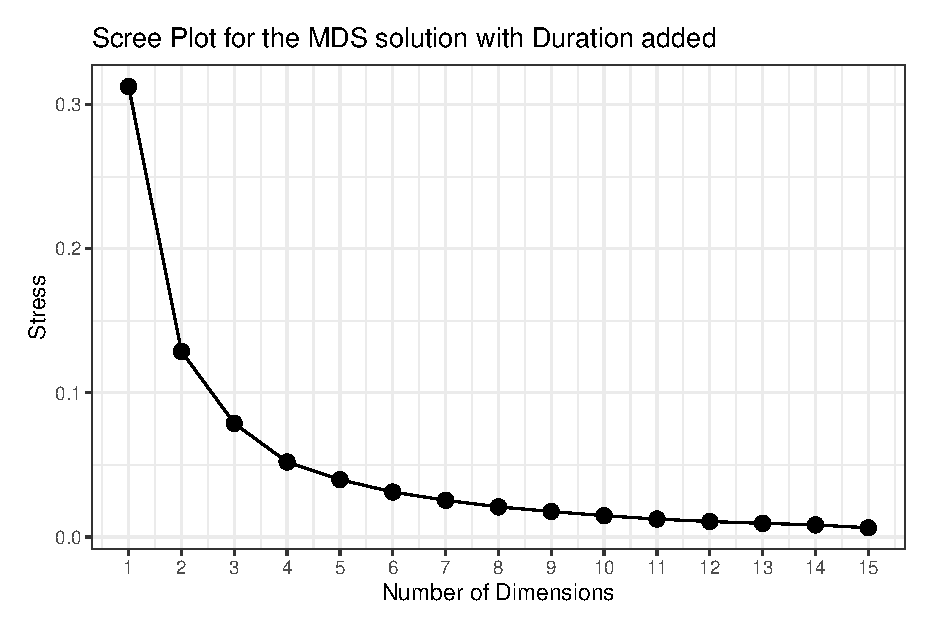
\includegraphics[width = 0.8\linewidth]{images/MDS/stress_plot_dur.eps}
\end{figure}
\end{frame}

\begin{frame}{Explanation of the plots}
  \begin{itemize}
    \item Each point $=$ unique speaker x phonation combination.
    \item Colors $=$ phonation type.
    \begin{itemize}
      \item Modal $=$ black
      \item Breathy $=$ orange
      \item Checked $=$ blue
      \item Rearticulated $=$ green
    \end{itemize}
    \item Axes $=$ dimensions of the acoustic space.
  \end{itemize}
\end{frame}

\begin{frame}{Dimensionality in SLZ}
  \begin{itemize}
    \item Scan the QR code to see the three-dimensional space.
    % \item Or use the link: \href{https://bit.ly/3St9S6g}{https://bit.ly/3St9S6g}
  \end{itemize}
  \begin{figure}[h!]
    \centering
    
\includegraphics[width=5cm, scale=0.5]{qrcode_3d_plot.eps}
  \end{figure}
\end{frame}

\begin{frame}{Takeaways from 3D plot}
  \begin{itemize}
    \item Shows clear groupings of phonation types 
    \item 
  \end{itemize}
\end{frame}

\begin{frame}{Dimensionality in SLZ}
  \begin{figure}
    \centering
    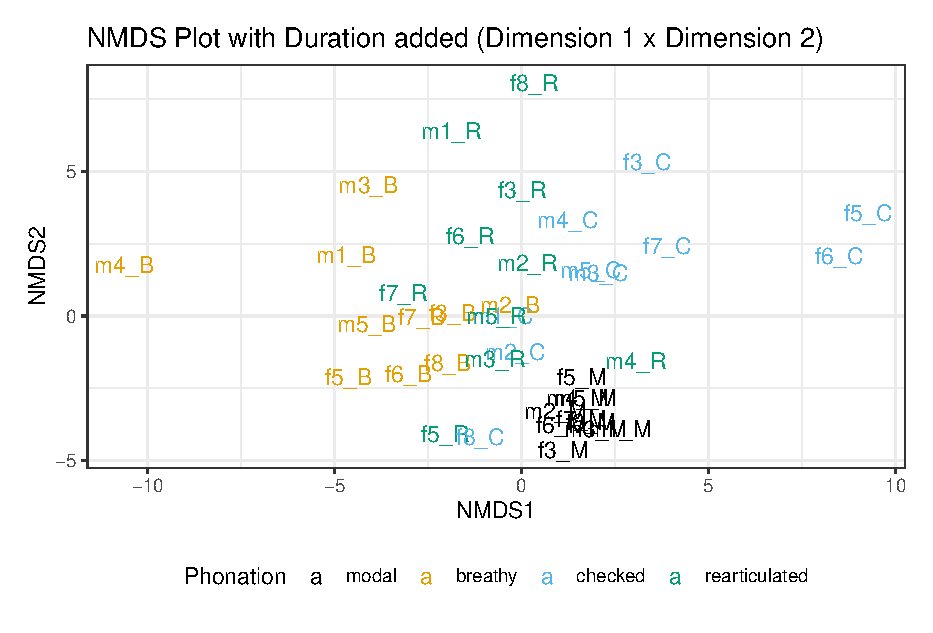
\includegraphics[width = 0.8\linewidth]{images/MDS/nmds12_dur.eps}
  \end{figure}
\end{frame}

\begin{frame}{Dimensionality in SLZ}
  \begin{figure}
    \centering
    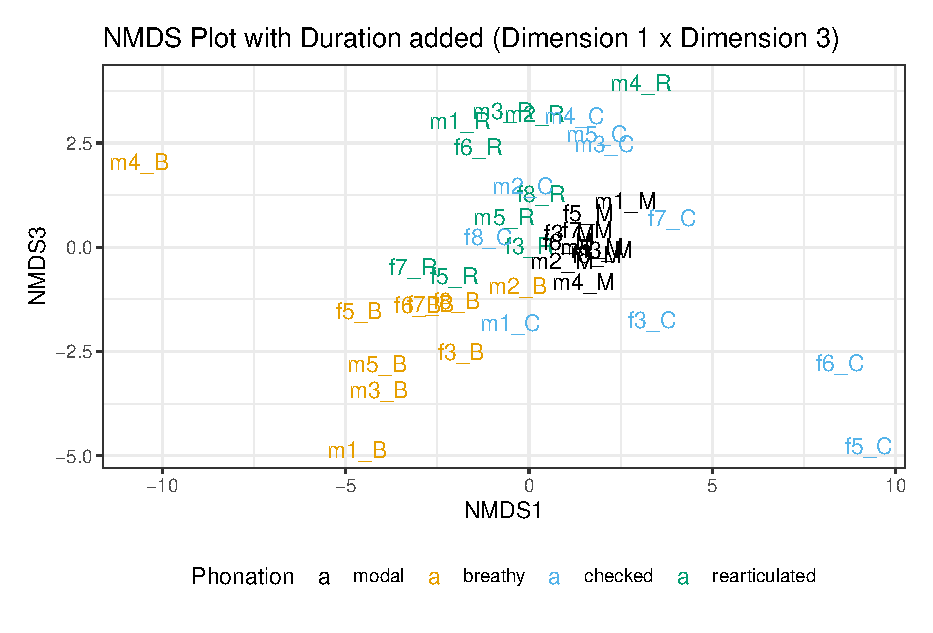
\includegraphics[width = 0.8\linewidth]{images/MDS/nmds13_dur.eps}
  \end{figure}
\end{frame}

\begin{frame}{Dimensionality in SLZ}
  \begin{figure}
    \centering
    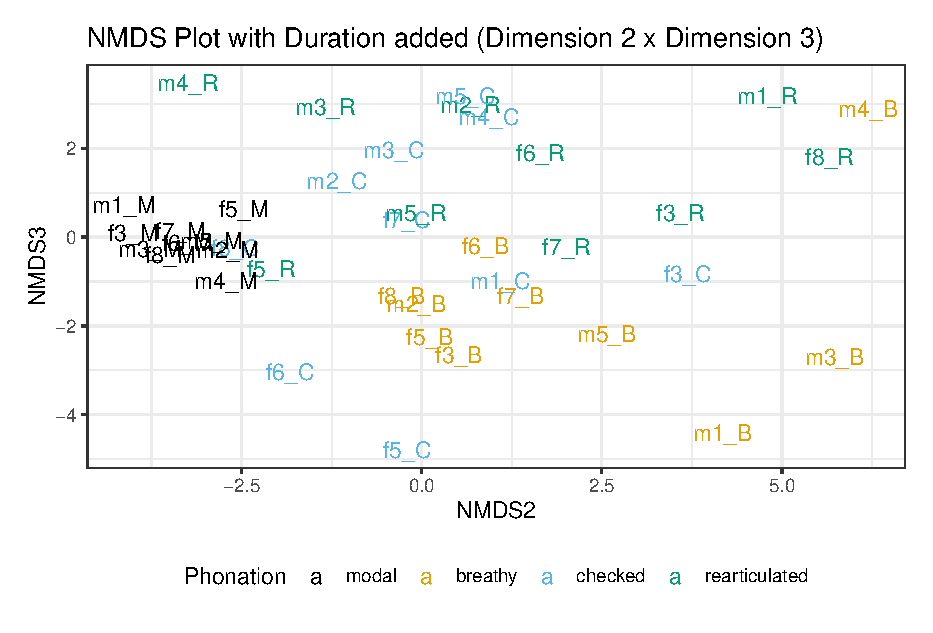
\includegraphics[width = 0.8\linewidth]{images/MDS/nmds23_dur.eps}
  \end{figure}
\end{frame}

\begin{frame}{Summary of Dimensions}
  \begin{itemize}
    \item Dimension 1 (D1) gives a rough continuum from breathy to creaky.
    \item Dimension 2 (D2) gives a rough continuum from modal to nonmodal.
    \item Dimension 3 (D3) gives a rough continuum from breathy to creaky.
  \end{itemize}
\end{frame}

\begin{frame}{Correlation to Acoustic Measures}
  \begin{itemize}
    \item D1 correlated with spectral tilt measures: 
    \begin{itemize}
      \item H1*$-$A1* ($r^2 = -0.83$) 
      \item H1*$-$A2* ($r^2 = -0.86$)
      \item H1*$-$A3* ($r^2 = -0.81$)
    \end{itemize}
    \item D2 correlated with periodicity and energy: 
    \begin{itemize}
      \item HNR\textless 500 Hz ($r^2 = -0.79$)
      \item HNR\textless 1500 Hz ($r^2 = -0.80$)
      \item Energy ($r^2 = -0.79$)
    \end{itemize}
    \item D3 correlated with spectral tilt:
    \begin{itemize}
      \item residual H1* ($r^2 = -0.72$)
      \item H2*$-$H4* ($r^2 = -0.69$)
      \item H2* ($r^2 = -0.68$)
    \end{itemize}
  \end{itemize}
\end{frame}

\begin{frame}{Summary of Acoustic Landscape}
  \begin{itemize}
    \item SLZ's phonation occupies a three-dimensional space.
    \item Dimensions are correlated with glottal-airflow continuum (D1/D3) and nonmodal-to-modal continuum (D2).
    \item Dimensions are similar to those found in \citet{keatingCrosslanguageAcousticSpace2023}.
  \end{itemize}
\end{frame}

%-----------------------------------------------------------
\subsection{Random Forests show important measures}
%-----------------------------------------------------------

\begin{frame}{What is a Random Forest?}
  \begin{itemize}
    \item Random Forest is a subclass of decision trees that uses an ensemble of decision trees to make predictions \citep{breimanClassificationRegressionTrees1986,breimanBaggingPredictors1996,breimanRandomForests2001}.
    \item More robust than 
  \end{itemize}
\end{frame}

\begin{frame}{Interpreting Random Forests}
  \begin{itemize}
    \item 
  \end{itemize}
\end{frame}

\begin{frame}
  \frametitle{Variable Importance}
  \begin{figure}[h!]
    \centering
    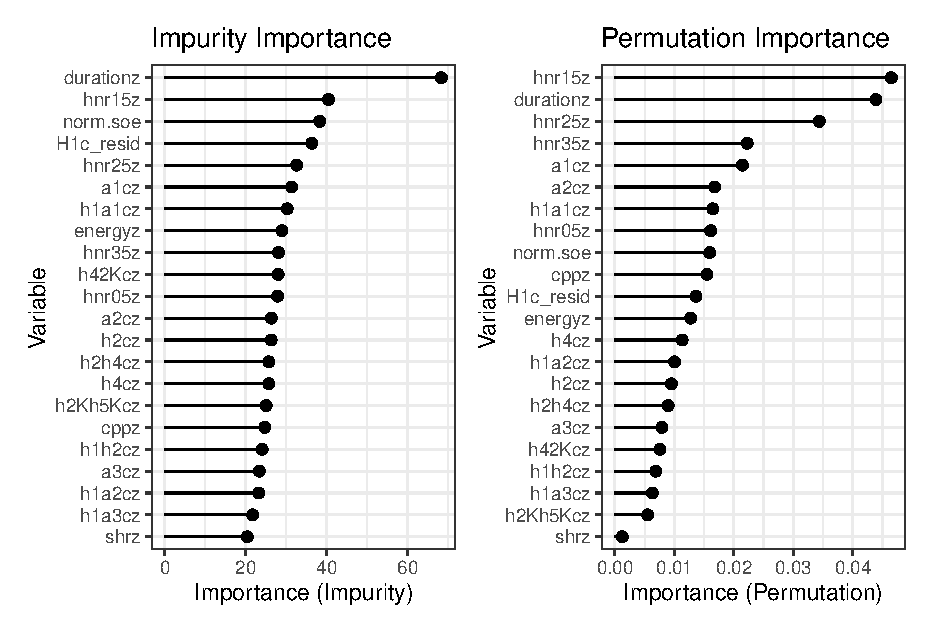
\includegraphics[width = 0.8\linewidth]{images/RandomForest/rf_dur_plots.eps}
  \end{figure}
\end{frame}

\begin{frame}{Variable Importance}
  \begin{itemize}
    \item Variable importance shows that only a handful of measures are important for capturing phonation contrasts.
    \begin{enumerate}
      \item Duration
      \item A1*
		  \item H1*$-$A1*
      \item Residual H1*
		  \item HNR < 1500 Hz
		  \item Strength of Excitation (SoE)
    \end{enumerate} 
  \end{itemize}
\end{frame}

\begin{frame}{Duration}
  \begin{figure}[h!]
    \centering
    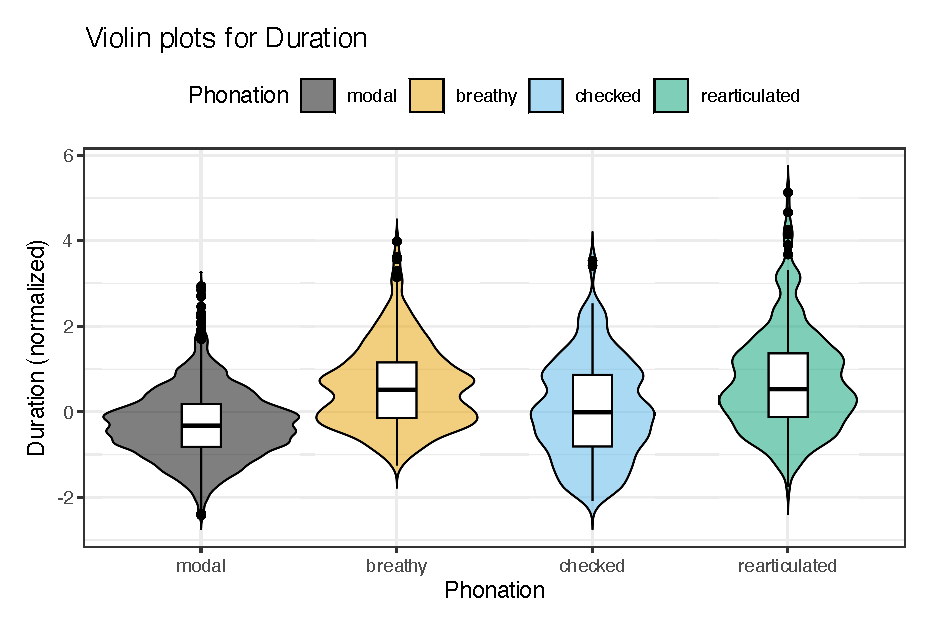
\includegraphics[width = 0.8\linewidth]{images/duration_plot.eps}
  \end{figure}
\end{frame}

\begin{frame}{A1*}
  \begin{figure}[h!]
    \centering
    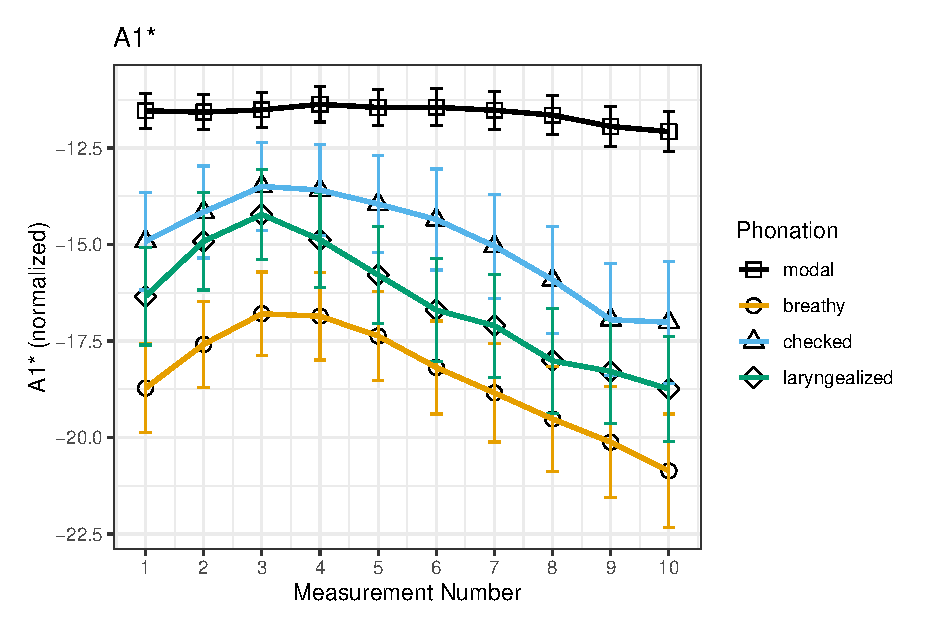
\includegraphics[width = 0.8\linewidth]{images/slz_a1c.eps}
  \end{figure}
\end{frame}

\begin{frame}{H1*$-$A1*}
  \begin{figure}[h!]
    \centering
    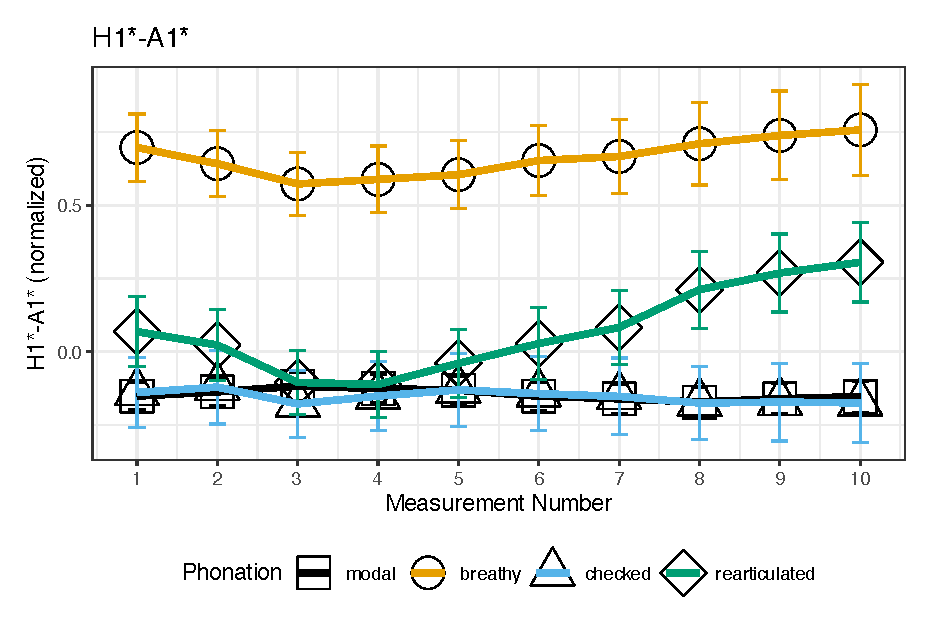
\includegraphics[width = 0.8\linewidth]{images/h1a1_line.eps}
  \end{figure}
\end{frame}

\begin{frame}{Residual H1*}
  \begin{figure}[h!]
    \centering
    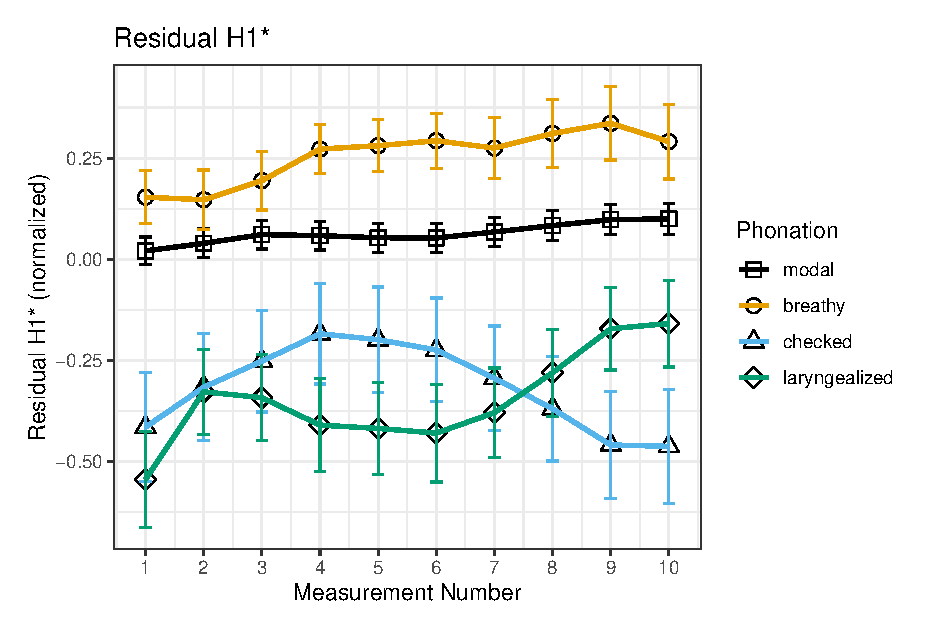
\includegraphics[width = 0.8\linewidth]{images/slz_residual_h1c.eps}
  \end{figure}
\end{frame}

\begin{frame}{HNR < 1500 Hz}
  \begin{figure}[h!]
    \centering
    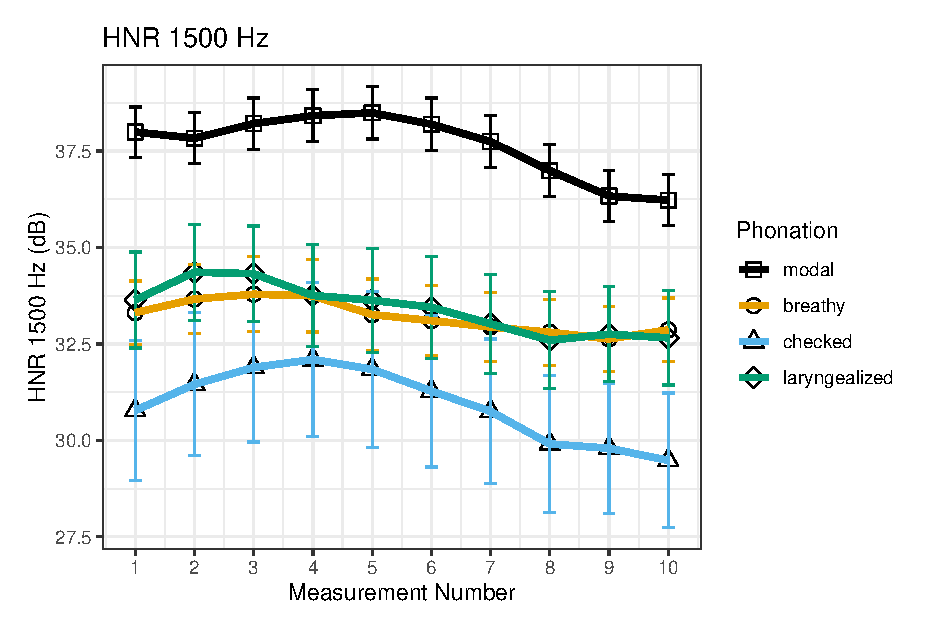
\includegraphics[width = 0.8\linewidth]{images/slz_hnr15.eps}
  \end{figure}
\end{frame}

\begin{frame}{Strength of Excitation (SoE)}
  \begin{figure}[h!]
    \centering
    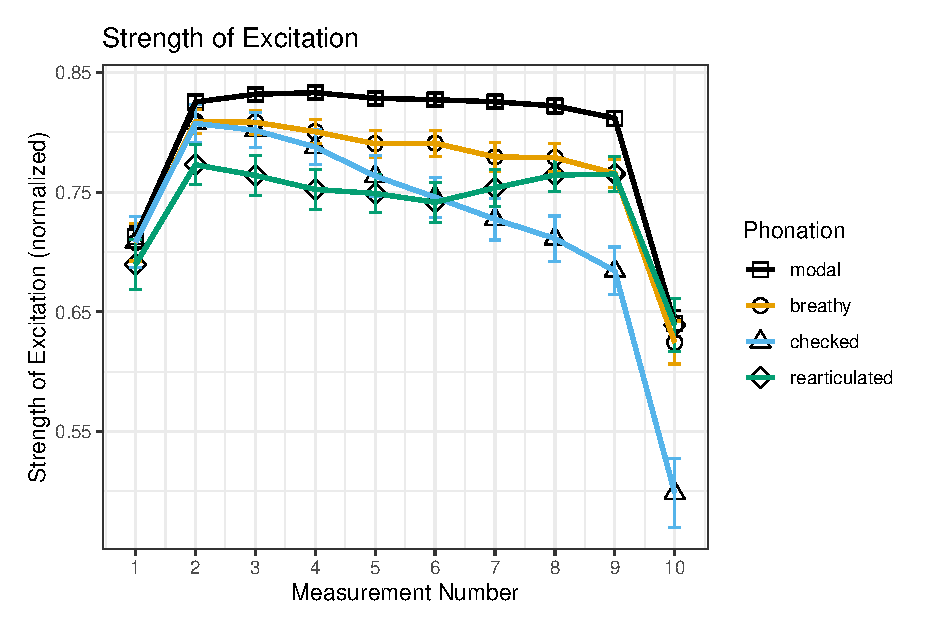
\includegraphics[width = 0.8\linewidth]{images/slz_soe.eps}
  \end{figure}
\end{frame}

\begin{frame}{Summary of Random Forest Results}
  \begin{itemize}
    \item Only a handful of measures are important for capturing phonation contrasts.
    \item Duration, A1*, H1*$-$A1*, residual H1*, HNR < 1500 Hz, and SoE are the most important measures.
    \item There is a lot of overlap between MDS' correlated measures and the important measures from the Random Forests.
  \end{itemize}
\end{frame}

%-----------------------------------------------------------
\subsection{Laryngeal Complexity in SLZ}
%-----------------------------------------------------------

\begin{frame}{Quanitfying Laryngeal Complexity}
  \begin{itemize}
    \item Laryngeal complexity is the number of phonation contrasts in a language.
    \item More phonation contrasts means more complex laryngeal system.
    \item Laryngeal complexity can be measured by the number of phonation contrasts in a language.
    \item Laryngeal complexity can be measured by the dimensionality of the acoustic space.
  \end{itemize}
\end{frame}

\begin{frame}{What are Generalized Additive Mixed Models (GAMMs)}
  \begin{itemize}
    \item GAMMs are a type of statistical model that can be used to analyze non-linear relationships between variables.
  \end{itemize}
\end{frame}

\begin{frame}{Evaluating GAMMs}
  \begin{itemize}
    \item Laryngeal complexity is measured by the number of phonation contrasts in a language.
    \item SLZ has four phonation contrasts.
    \item The more phonation contrasts a language has, the more complex its laryngeal system is.
  \end{itemize}
\end{frame}

\begin{frame}{Model fit for \textit{f}0}
  \begin{figure}[h!]
    \centering
    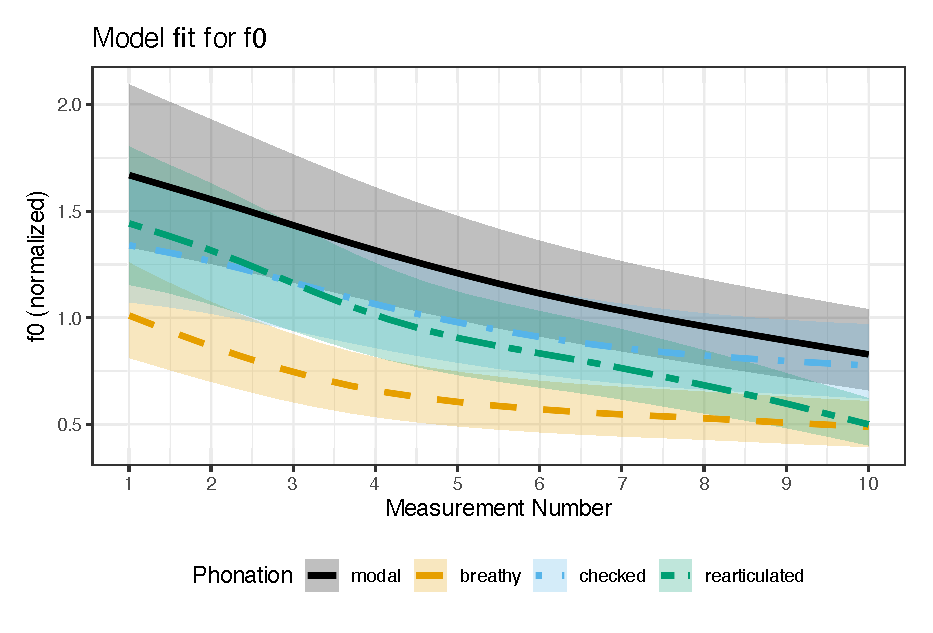
\includegraphics[width = 0.8\linewidth]{images/LCH_GAMMs/f0_model_fit.eps}
  \end{figure}
\end{frame}

\begin{frame}{Model difference for \textit{f}0}
  \begin{figure}[h!]
    \centering
    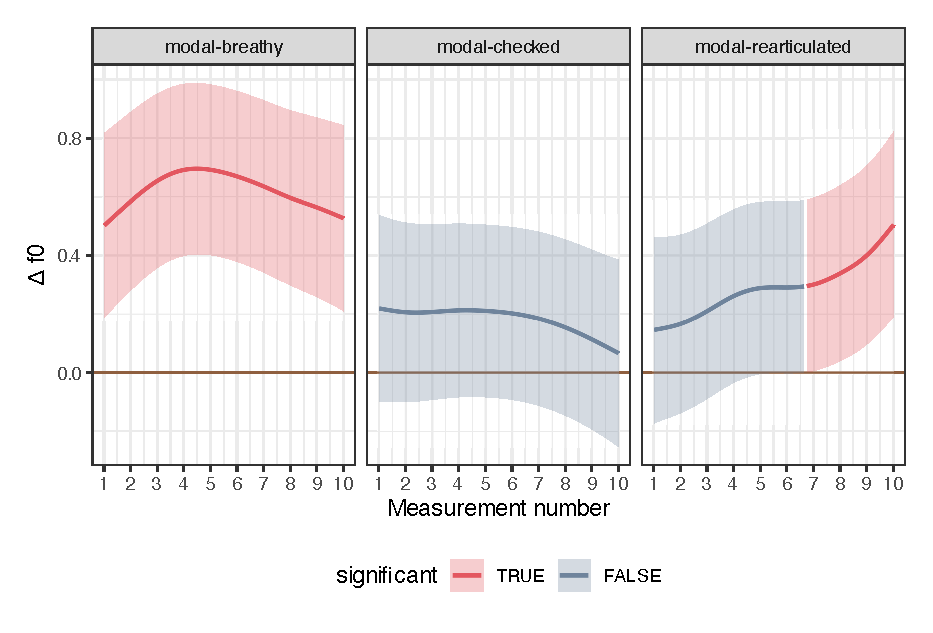
\includegraphics[width = 0.8\linewidth]{images/LCH_GAMMs/f0_model_diff.eps}
  \end{figure}
\end{frame}

\begin{frame}{Model fit for HNR}
  \begin{figure}[h!]
    \centering
    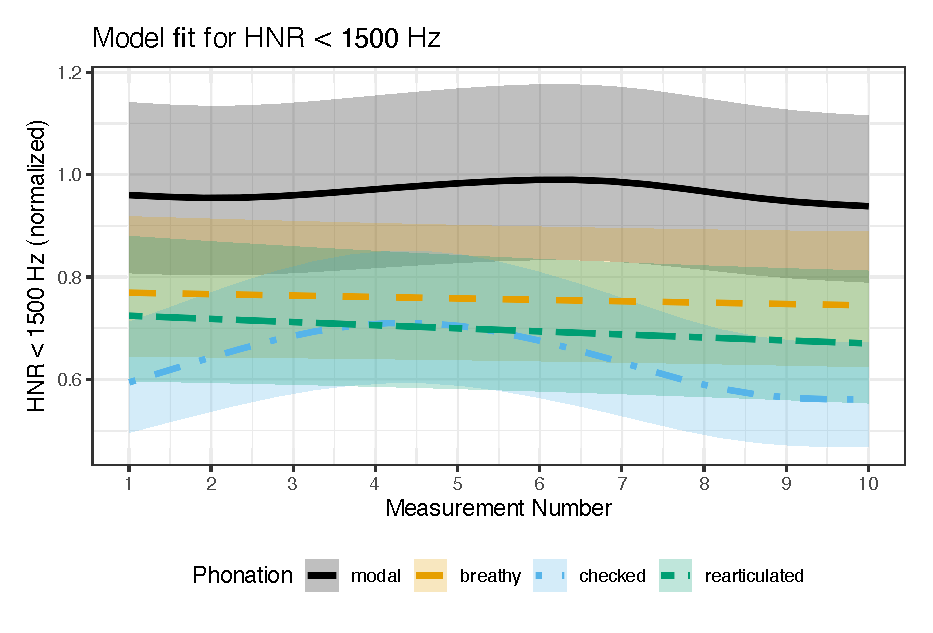
\includegraphics[width = 0.8\linewidth]{images/LCH_GAMMs/hnr15_model_fit.eps}
  \end{figure}
\end{frame}

\begin{frame}{Model difference for HNR}
  \begin{figure}[h!]
    \centering
    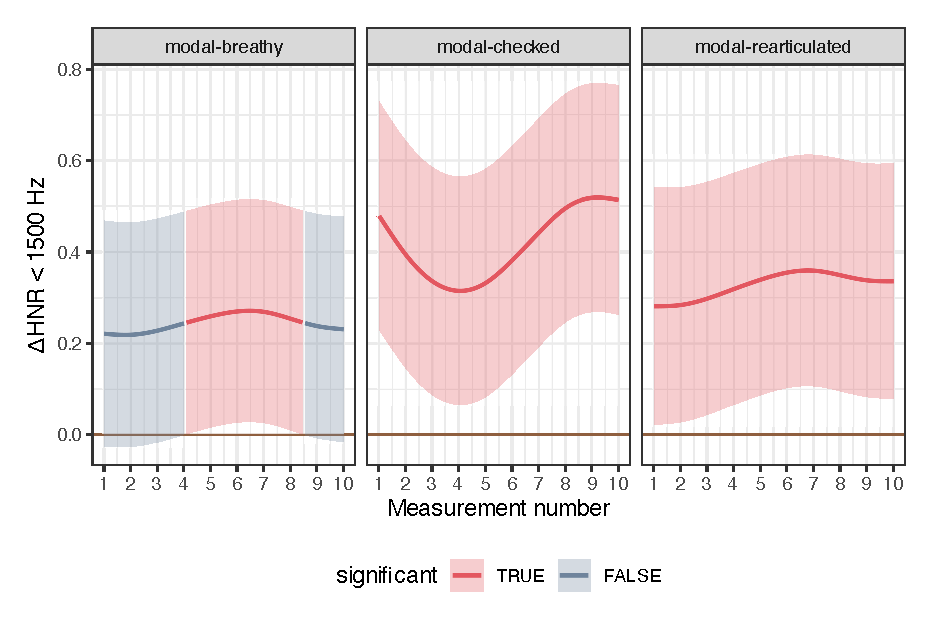
\includegraphics[width = 0.8\linewidth]{images/LCH_GAMMs/hnr15_model_diff.eps}
  \end{figure}
\end{frame}

\begin{frame}{Model fit for SoE}
  \begin{figure}[h!]
    \centering
    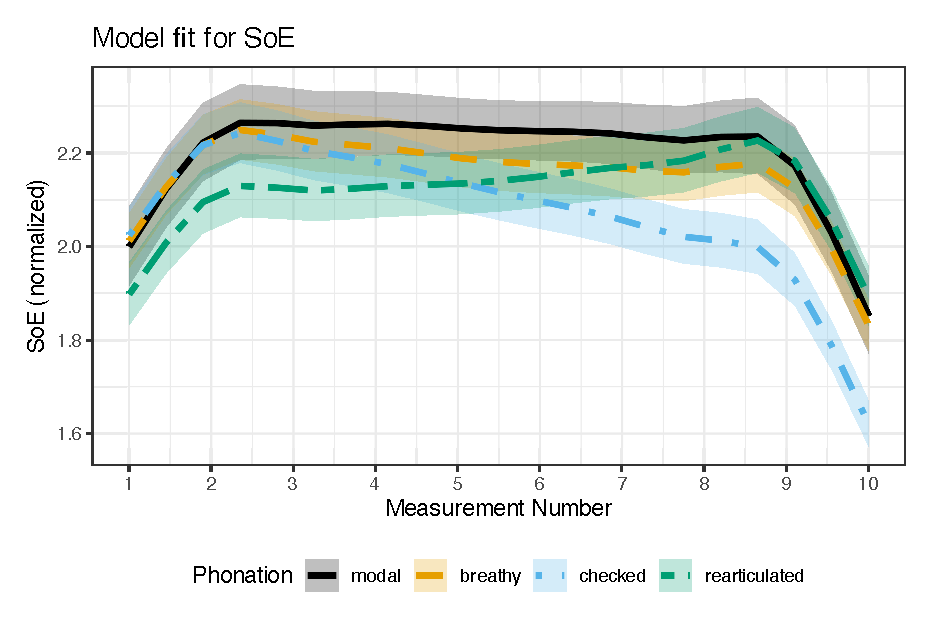
\includegraphics[width = 0.8\linewidth]{images/LCH_GAMMs/soe_model_fit.eps}
  \end{figure}
\end{frame}

\begin{frame}{Model difference for SoE}
  \begin{figure}[h!]
    \centering
    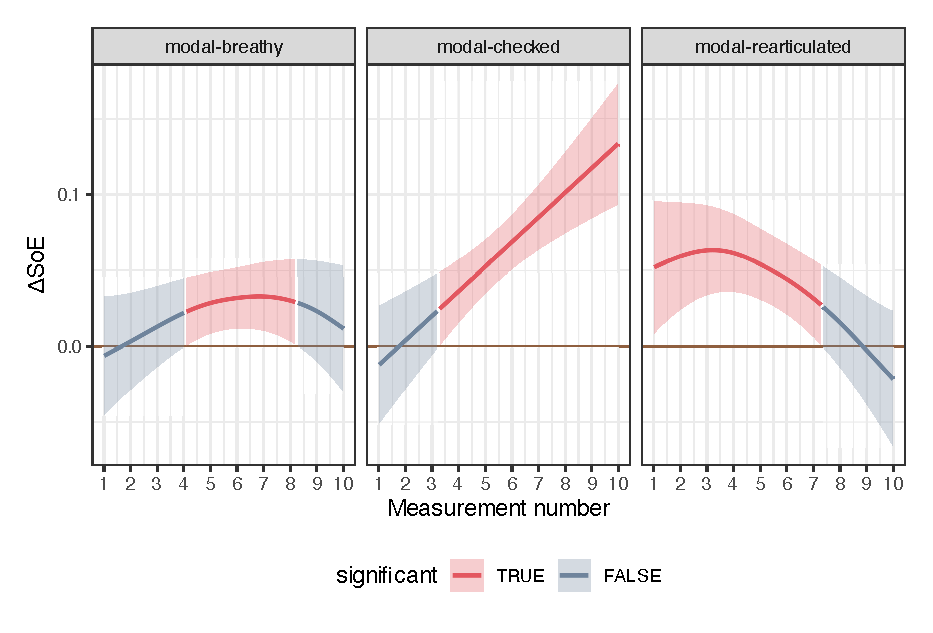
\includegraphics[width = 0.8\linewidth]{images/LCH_GAMMs/soe_model_diff.eps}
  \end{figure}
\end{frame}

\begin{frame}{Summary of Laryngeal Complexity}
  \begin{itemize}
    \item SLZ has four phonation contrasts.
    \item SLZ's phonation occupies a three-dimensional space.
    \item Dimensions are correlated with glottal-airflow continuum (D1/D3) and nonmodal-to-modal continuum (D2).
    \item Dimensions are similar to those found in \citet{keatingCrosslanguageAcousticSpace2023}.
  \end{itemize}
\end{frame}

%-----------------------------------------------------------
\section{Summary and conclusions}
%-----------------------------------------------------------
\begin{frame}{Summary of Results}
  \begin{itemize}
    \item SLZ's phonation occupies a three-dimensional space.
    \item Dimensions are correlated with glottal-airflow continuum (D1/D3) and nonmodal-to-modal continuum (D2).
    \begin{itemize}
      \item Collaborated with acoustic measure correlations.
    \end{itemize}
    \item Dimensions are similar to those found in \citeauthor{keatingCrosslanguageAcousticSpace2023}.
  \end{itemize}
\end{frame}

\begin{frame}{Summary}
  \begin{itemize}
    \item Acoustic space can be reduced to two dimensions.
    \item More dimensions add more information about these two dimensions.
  \end{itemize}
  \begin{figure}[h!]
    \centering
    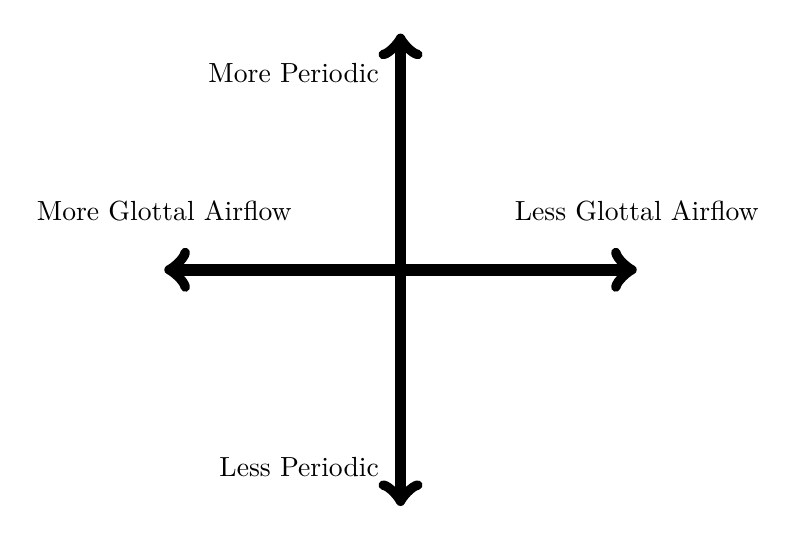
\begin{tikzpicture}
        % Draw the horizontal line with arrows
        \draw[<->, line width=1.5mm] (-3,0) -- (3,0);
        % Draw the vertical line with arrows
        \draw[<->, line width=1.5mm] (0,-3) -- (0,3);
        
        % Labels for the horizontal line
        \node[below,yshift=1cm] at (-3,0) {More Glottal Airflow};
        \node[below,yshift=1cm] at (3,0) {Less Glottal Airflow};
        
        % Labels for the vertical line
        \node[left, xshift = -1.5mm] at (0,-2.5) {Less Periodic};
        \node[left, xshift = -1.5mm] at (0,2.5) {More Periodic};
    \end{tikzpicture}
\end{figure}
\end{frame}

\begin{frame}{Summary}

  % Keep the summary *very short*.
  \begin{itemize}
  \item Dimensionality reduction also occurs in a single language.
  \item Dimensions correspond to glottal-airflow and nonmodal-to-modal continua within a language and cross-linguistically.
  \item If additional dimensions are added, they only add additional information about these two dimension.
  \end{itemize}
  
  % The following outlook is optional.
  \vskip0pt plus.5fill
  \begin{itemize}
  \item
    Outlook
    \begin{itemize}
    \item What are the perceptual cues that speakers use to distinguish between phonation types?
    \item How do these dimensions relate to the phonology?
    \end{itemize}
  \end{itemize}
\end{frame}

\begin{frame}
  \frametitle{Duxhklhenhu' lhe' (Thank you)}
  \begin{figure}[h!]
    \centering
    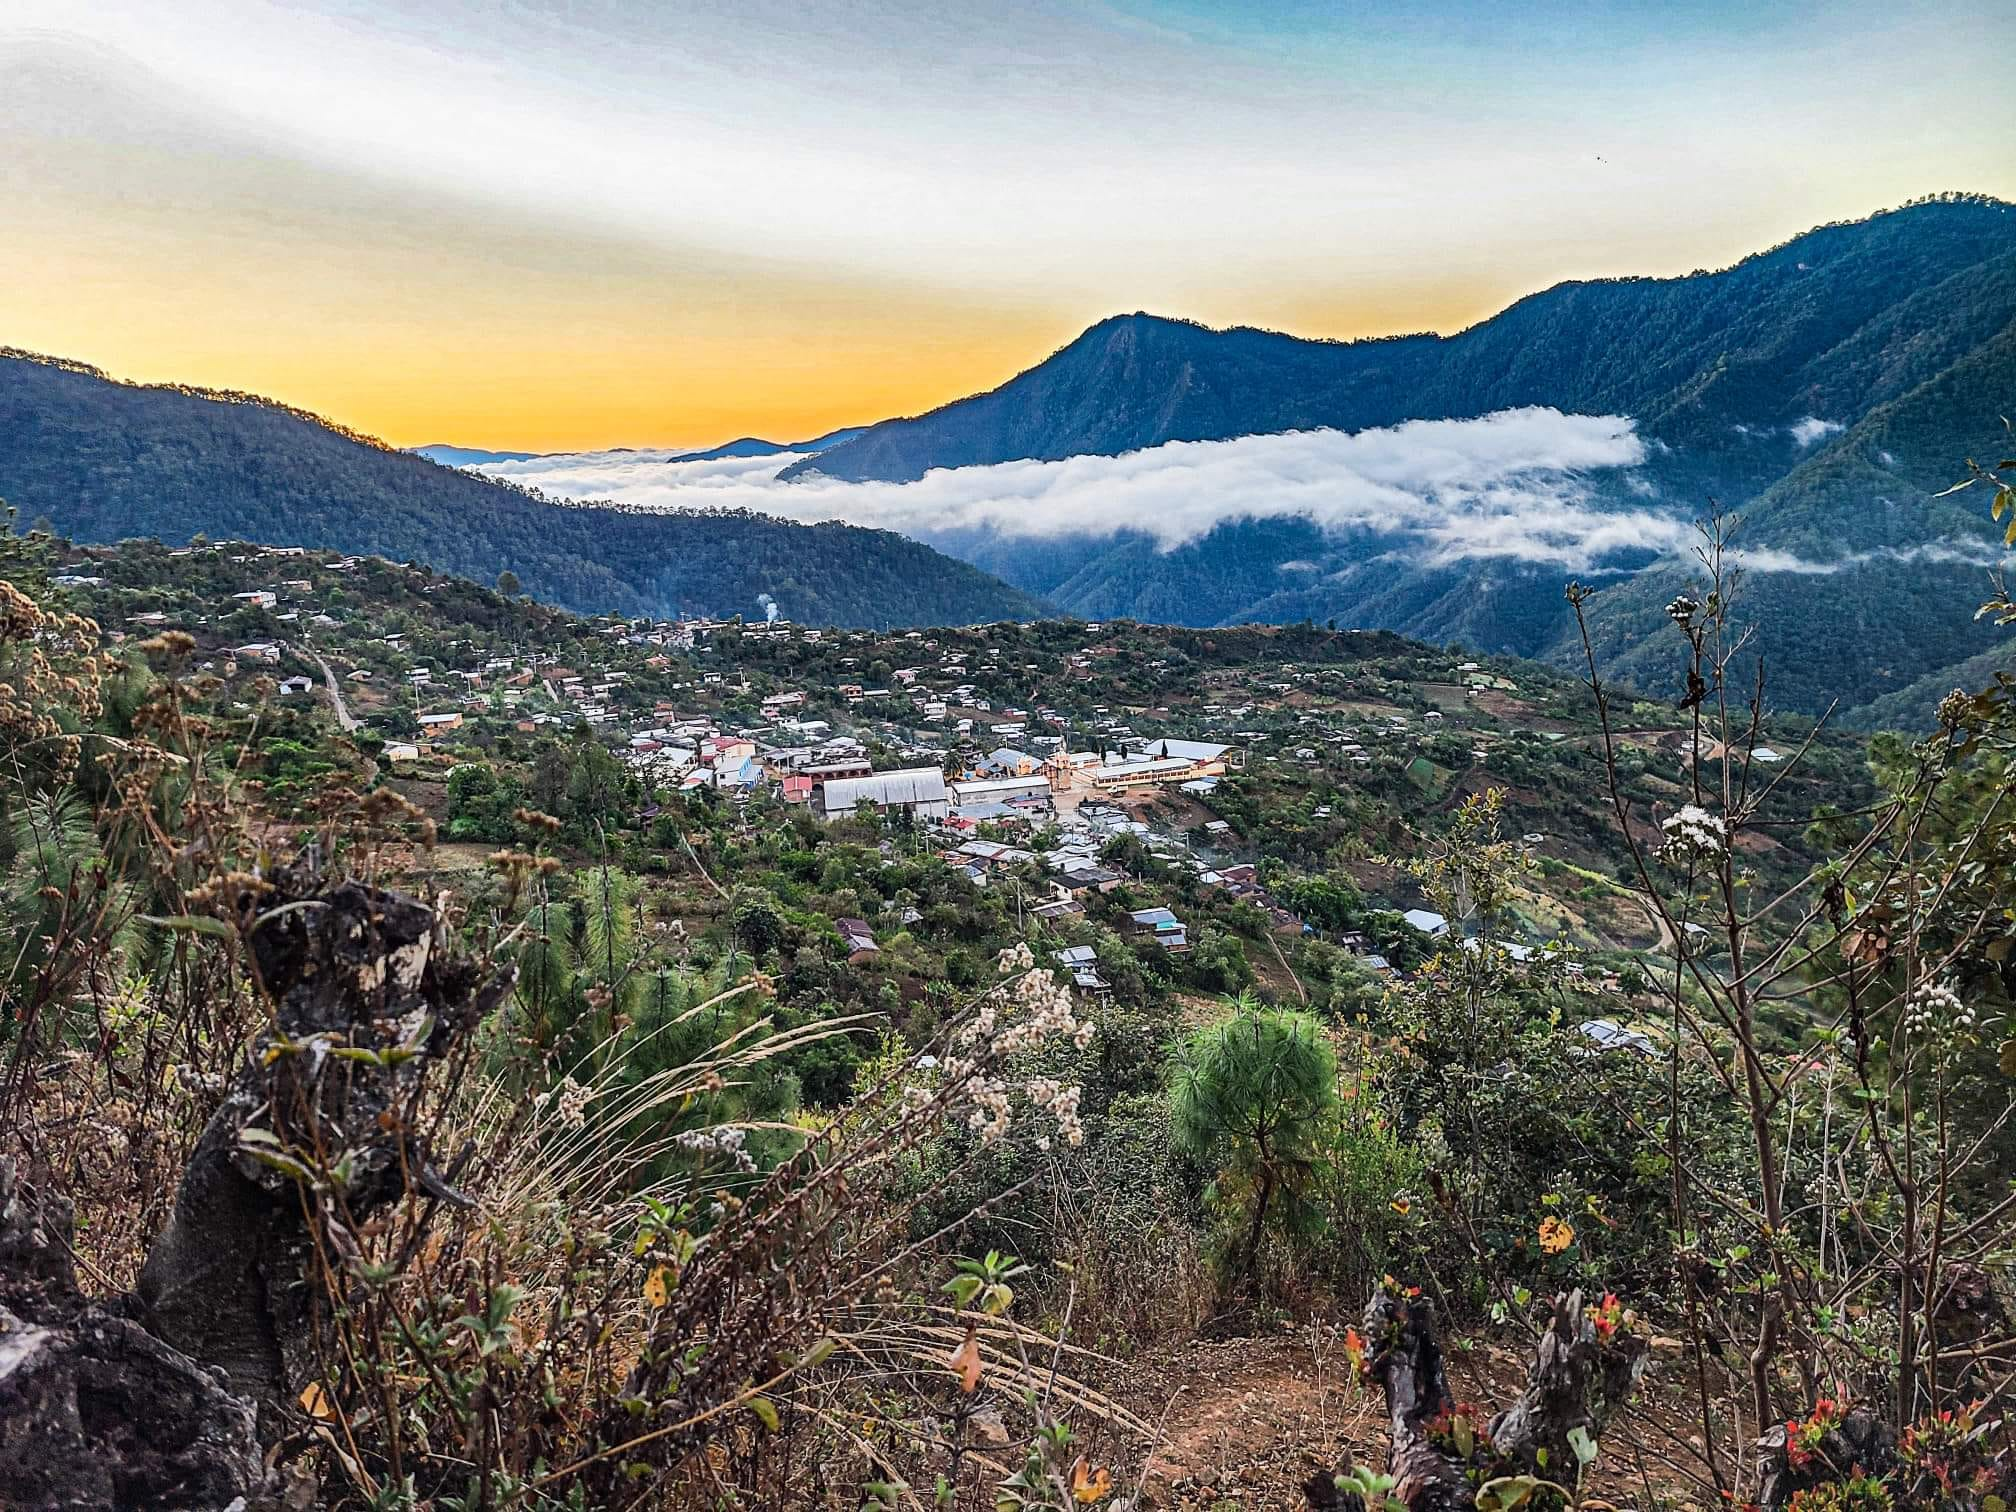
\includegraphics[width = \linewidth]{images/SantiagoLaxopa.jpeg}
  %   \label{fig:fieldwork}
  \end{figure}
\end{frame}

%-----------------------------------------------------------
\section*{Acknowledgements}
%-----------------------------------------------------------

\begin{frame}
  \frametitle{Acknowledgements}
  \begin{itemize}
    \item Thank you to the speakers in Santiago Laxopa for sharing their time and language expertise. 
    \item Thank you to my Grant McGuire, Jaye Padgett, Marc Garellek, Ryan Bennett, Jack Duff, Maya Wax Cavallaro, and many others for their help and discussions during all stages of this project. 
  \end{itemize}
\end{frame}

\begin{frame}
  \frametitle{Acknowledgements}
  This work is supported by funding from: 
  \begin{itemize}
    \item The National Science Foundation under Grant No. 2019804
    \item The Humanities Institute at UC Santa Cruz 
    \item The Jacobs Research Funds
  \end{itemize}

\end{frame}


\appendix
%-----------------------------------------------------------
\section<presentation>*{\appendixname}
%-----------------------------------------------------------
%-----------------------------------------------------------
\section{References}
%-----------------------------------------------------------
\begin{frame}[t,allowframebreaks]
  \frametitle{References}
    \printbibliography
\end{frame}



\end{document}